\documentclass[11pt]{article}
\usepackage[margin=1.1in]{geometry}
\usepackage[T1]{fontenc}
\usepackage{amsmath,amssymb,amsthm}
\usepackage{booktabs}
\usepackage{xcolor}
\definecolor{linknavy}{RGB}{25, 55, 125}
\usepackage[colorlinks=true, linkcolor=linknavy, citecolor=linknavy, urlcolor=linknavy, hypertexnames=false]{hyperref}
\usepackage{array}
\usepackage[justification=raggedright,singlelinecheck=false]{caption}
\usepackage{orcidlink}
\usepackage{fancyhdr}
\usepackage{algorithm}
\usepackage{algpseudocode}
\usepackage{pgfplots}
\pgfplotsset{compat=1.16}
\makeatletter\g@addto@macro\UrlBreaks{\do\-\do\_}\makeatother

\newtheorem{theorem}{Theorem}[section]
\newtheorem{proposition}[theorem]{Proposition}
\newtheorem{lemma}[theorem]{Lemma}
\theoremstyle{definition}
\newtheorem{definition}[theorem]{Definition}
\theoremstyle{remark}
\newtheorem{remark}[theorem]{Remark}

% Numbers quoted in the text that are read from stored records by gen_tables.py.
% BEGIN GENERATED macros
\newcommand{\numAtlasTrapMax}{20}
\newcommand{\numAtlasTrapRun}{bicorner-opp}
\newcommand{\numAtlasCertMin}{67}
\newcommand{\numAtlasCertMinRun}{fa2b-residue}
\newcommand{\numAtlasCertMax}{97}
\newcommand{\numAtlasCertMaxRun}{core}
\newcommand{\numCertNzMin}{6}
\newcommand{\numCertNzMax}{11}
\newcommand{\numRatioMin}{0.3}
\newcommand{\numRatioMax}{2.1}
\newcommand{\numSingMin}{0.4}
\newcommand{\numSingMax}{0.6}
\newcommand{\numChamberTotal}{125{,}097{,}984}
\newcommand{\numChamberUnit}{2{,}843{,}136}
\newcommand{\numGenSoneMin}{49}
\newcommand{\numGenSoneMax}{95}
\newcommand{\numGenStwoMin}{241}
\newcommand{\numGenStwoMax}{2224}
\newcommand{\numAtlasRuns}{9}
\newcommand{\numAtlasLeaves}{1{,}397{,}962}
\newcommand{\numAtlasBall}{10}
\newcommand{\numAtlasCertShare}{86}
\newcommand{\numPolyFiveOne}{35}
\newcommand{\numPolyFiveTwo}{25}
\newcommand{\numPolyFourOne}{19}
% END GENERATED macros

% Avoid single lines stranded at the top or bottom of a page.
\widowpenalty=10000
\clubpenalty=10000

% Evidence marks. [MV] machine-verified (exact arithmetic, or a recorded check that can fail);
% [D] derived in the text or in a written derivation of the experiment records;
% [V] read on the primary source; [U] not confirmed on a primary source.
\newcommand{\mk}[1]{\,{\scriptsize[#1]}}
\newcolumntype{L}[1]{>{\raggedright\arraybackslash}p{#1}}
\newcommand{\MV}{\mk{MV}}
\newcommand{\Dm}{\mk{D}}
\newcommand{\Vm}{\mk{V}}
\newcommand{\Um}{\mk{U}}

% Page-1 header block (conventions/manuscript-header-standard.md). The four document
% macros are set by the publishing tool when the version DOI is reserved.
\newcommand{\doctype}{Preprint}
\newcommand{\docversion}{v0.12}
\newcommand{\docdate}{14 November 2026}
\newcommand{\versiondoi}{10.5281/zenodo.23887585}
\newcommand{\conceptdoi}{10.5281/zenodo.21542483}
\newcommand{\docrepo}{github.com/fsantibanezleal/CAOS\_RESEARCH}
\newcommand{\headerblock}{%
\begin{center}
\fbox{\parbox{0.94\textwidth}{\small\raggedright
\textbf{\doctype} \quad$\cdot$\quad \docversion, \docdate \quad$\cdot$\quad Licence CC BY 4.0\\[2pt]
CAOS Research open-problems programme \quad$\cdot$\quad problem \texttt{central-configurations}\\[2pt]
Version DOI \href{https://doi.org/\versiondoi}{\texttt{\versiondoi}} \quad$\cdot$\quad
concept DOI (always latest) \href{https://doi.org/\conceptdoi}{\texttt{\conceptdoi}}\\[2pt]
Not peer reviewed. Source code, data and computational records: \href{https://\docrepo}{\texttt{\docrepo}}
}}
\end{center}
\vspace{4pt}}

\title{Replication and screening of tropical finiteness certificates for central
configurations, with exact comet decisions and the status of a six-body symmetric stratum}
\author{Felipe Santib\'a\~nez-Leal\,\orcidlink{0000-0002-0150-3246}\\
\small CAOS Research program, \texttt{github.com/fsantibanezleal/CAOS\_RESEARCH}}
\date{\docdate}

\pagestyle{fancy}
\fancyhf{}
\fancyhead[L]{\small CAOS Research \doctype}
\fancyhead[R]{\small Tropical Certificates for Central Configurations \textperiodcentered\ \docversion}
\fancyfoot[C]{\small \thepage}
\fancypagestyle{plain}{\fancyhf{}\fancyfoot[C]{\small \thepage}\renewcommand{\headrulewidth}{0pt}}

\begin{document}
\maketitle
\thispagestyle{plain}
\headerblock

\begin{abstract}
We report a replication and screening study around Smale's 6th problem (finiteness of planar
central configurations). Conclusions rest on exact rational or integer arithmetic, with three
stated exceptions: the \texttt{gfan} prevariety runs use the machine-integer fast path (the
overflow-checked rerun has not been made), the random linear section probes are probabilistic,
and the modular Gr\"obner screens are used for triage only. The contributions are:
(i) an exact calibration of the Albouy--Chenciner mutual-distance equations in open tooling,
including a machine rediscovery of their dimension-blindness (the regular tetrahedron coexists
with the square in the equal-mass rhombus stratum of the 4-body distance system until the
Cayley--Menger equation is adjoined; under the normalization that fixes the force constant to
the total mass, the square, with side $a$ satisfying $a^3=(4+\sqrt2)/8$, the larger of the two
positive roots of $32a^6-32a^3+7=0$, is then the unique positive point of the stratum);
(ii) a machine measurement of the \emph{enrichment law}: adjoining the asymmetric (Roberts)
equations and the energy--inertia relation renders the $n=3$ distance ideal zero-dimensional
directly;
(iii) an independent reproduction of the Jensen--Leykin tropical prevariety certificate of
generic-mass finiteness for $n=5$ (arXiv:2301.02305v2): both published $f$-vectors match digit
for digit and the pointedness of the recession cone is verified by an independent exact parser,
on the fast path; the same binary in arbitrary precision reproduces the three $n=4$
$f$-vectors it shares with the screening;
(iv) a screening over mass-valuation families and equation-system variants at $n=4,5$ with
complete tables, which finds two new working valuation families beyond the two published,
replicates generic-mass finiteness for $n=4$ purely polyhedrally in seconds, and shows that
removing the ten dependent symmetric Albouy--Chenciner equations destroys the certificate at
every tested valuation; every comet is decided exactly by a rational-arithmetic feasibility
certificate, and adding valid equations is measured separately (Dziobek's equations are
tropically active but not decisive at the hard case; the energy--inertia relation is inert);
(v) a status report on the two-pair reflection-symmetric stratum of the six-body problem:
the cases $k=0,1,2,4$ of a fibre-dimension chain are proved with written proofs, the case
$k=3$ is reduced to four bilinear conditions, an interval atlas certifies every region except
one exact degenerate point (the cross point) and one chart region still open, the degenerate
set of the cross family is finite, and no finiteness statement is claimed for the stratum; and
(vi) an audit of the Lean formalization of the five-body finiteness claims: its main theorem
states exactly the classical claim, and a scan of nine kernel-bypass patterns over 2,751 stored
and 85,756 generated modules finds none of them, which does not replace the kernel check.
The finiteness theorems replicated are due to Hampton--Moeckel, Albouy--Kaloshin and
Jensen--Leykin; the measurements in (i), (ii) and (iv) are, to our knowledge, new at this level
of explicitness, a statement not confirmed by a systematic literature search.
\end{abstract}

\section{Introduction}

A \emph{central configuration} (CC) of the Newtonian $n$-body problem with
masses $m_1,\dots,m_n>0$ is a configuration $x=(x_1,\dots,x_n)$,
$x_i\in\mathbb{R}^d$, satisfying
\begin{equation}
\lambda\,(x_i-c)=\sum_{j\neq i}\frac{m_j (x_j-x_i)}{r_{ij}^3},\qquad
i=1,\dots,n,
\end{equation}
for some $\lambda$, where $c$ is the center of mass and $r_{ij}=|x_i-x_j|$.
Smale's 6th problem for the 21st century \cite{Smale98} asks, following Chazy
\cite{Chazy18} and Wintner \cite{Wintner41}, whether for every $n$ and every
choice of positive masses the number of \emph{planar} central configurations,
up to symmetry, is finite. The problem text was read in the author's second version
of 7 August 1998; the journal printing was not read\Vm.

\paragraph{Evidence marks.}
Statements carry one of four marks. \MV\ marks a statement machine-verified in exact arithmetic,
or by a recorded check that can fail; \Dm\ a statement derived in the text or in a written
derivation held in the experiment records; \Vm\ a statement read on the primary source; \Um\ a
statement not confirmed on a primary source. A statement is called \emph{proved} only when the
paper gives its proof or points to a written proof in the records by file and line range;
otherwise it is stated as the records state it (reduced, claimed, open, dropped). Records are
cited relative to \path{problems/dynamical-systems/central-configurations/}, abbreviated
\texttt{CC/}; \texttt{EXP-NNN} names an experiment folder in \texttt{CC/experiments/}.

\paragraph{The ladder.}
For $n=4$ the number is finite for all positive masses (Hampton--Moeckel \cite{HM06}:
computer-assisted BKK certificate, count in $[32,8472]$\Vm; for the Dziobek configurations of the four-body problem
Dias \cite{Dias26} later gives a B\'ezout-type bound of 8192 for homogeneous potentials, from the abstract\Vm). For $n=5$ it
is finite except possibly on an explicit
codimension-two subvariety of mass space (Albouy--Kaloshin \cite{AK12}\Vm, from the abstract and
pp.~535--540); Moczurad and Zgliczy\'nski \cite{MZ26} give a computer-assisted exact count of the classes
for several mass sets that are exceptional for that result (from the abstract\Vm). Finiteness for $n=5$ and \emph{all} positive masses was claimed in October 2026
by three groups, one with a Lean formalization (Section~\ref{sec:five})\Vm; none of the claims
is refereed. The spatial 5-body Dziobek case is handled generically by Moeckel \cite{Moeckel01}
and explicitly by Hampton--Jensen \cite{HJ11}\Vm; Dias \cite{Dias17} extends generic finiteness of Dziobek
configurations to semi-integer exponents\Um. The case $n=6$ is open, reduced by
Chang--Chen \cite{ChangChen23} to twenty-four unsolved zw-diagram cases (their programme
preprint states the count verbatim, read on pages 1 to 6\Vm); for \emph{generic} masses the
purely polyhedral certificate of Jensen--Leykin \cite{JL25}\Vm, complete through $n=5$, is the
live frontier, and a six-body symmetric stratum is treated in Section~\ref{sec:stratum}.
Rigorous equal-mass censuses for $n\le 7$ are due to Moczurad--Zgliczy\'nski \cite{MZ19}\Vm, who also list
the equal-mass spatial configurations for $n=5,6$ \cite{MZ20}\Vm;
with one negative mass a continuum exists (Roberts \cite{Roberts99}\Vm, masses
$(1,1,1,1,-1/4)$), so positivity is essential.

\paragraph{Scope.}
This is a replication and screening study: it places the certificates of this ladder inside
one open, reproducible toolchain with stored artifacts, and then runs the experiments that
the frontier papers themselves call for. Since the five-body claims of 2026, the $n=5$
computations are no longer a route to a new theorem; they remain a replication, a screening of
the method, and the calibration for the open case $n=6$. Negative and capped results are
reported with the positive ones.

\section{Instruments and provenance}\label{sec:methods}

\subsection{Tool versions and recorded hashes}

\begin{table}[t]\centering\footnotesize
\begin{tabular}{@{}L{1.4cm}L{5.4cm}L{5.2cm}@{}}
\toprule
Tool & Release and build & Recorded SHA-256 \\
\midrule
\texttt{gfan} & 0.7, author tarball, two-line \texttt{\#include <cstdint>} patch for gcc~13, GMP, cddlib; WSL2 Ubuntu 24.04 & tarball and binary: not in the committed artifacts (UNVERIFIED) \\
\texttt{gfan} & 0.8beta, author tarball, same patch; binary installed as \texttt{gfan08} & tarball \texttt{fa7884e5f317c50f}, binary \texttt{0f177e6a4f7829fc} (prefixes) \\
\texttt{msolve} & 0.10.1, built in WSL & binary \texttt{be6ea2289f0fab9847bf} (prefix) \\
Singular & 4.3.2, Ubuntu 24.04 package & binary \texttt{90ab699b7a28486944a1} (prefix) \\
\texttt{sympy} & 1.14, Python 3.13 (exact layer) & not applicable \\
\bottomrule
\end{tabular}
\caption[Tools, builds and recorded hashes.]{Tools, builds and recorded hashes. The prefixes are the first hexadecimal digits
of the SHA-256 values in \path{CC/experiments/EXP-005-n6-prevariety-pow3/run08.sh},
\path{EXP-006-msolve-census/verdict.md} and \path{EXP-012-partial-gb-engine-spike/hypothesis.md}. % voice-ok
The experiment record for the $n=5$ reproduction states that the \texttt{gfan} 0.7 tarball
and binary hashes were recorded in an artifacts file; that file is absent from the
repository tree, so the values are not reproduced here.}\label{tab:tools}
\end{table}

The hashes of the 16 \texttt{gfan} inputs and 16 outputs of the screening grid are stored in
\path{CC/experiments/EXP-004-valuation-equation-screening/artifacts/hashes.txt}
(Table~\ref{tab:hashes} reproduces the six cells of system S1 at $n=5$).

\begin{table}[t]\centering\footnotesize
% BEGIN GENERATED table-hashes
\begin{tabular}{@{}lll@{}}
\toprule
Cell (system S1, $n=5$) & gfan input, SHA-256 prefix & gfan output, SHA-256 prefix \\
\midrule
powers of 3 & \texttt{632a79188e206f50} & \texttt{4ec34432160d2241} \\
squares & \texttt{4f69cdd0798298bd} & \texttt{c8500283d31e3891} \\
powers of 2 & \texttt{301ba5356dc79f5a} & \texttt{37c3c5dd73f958d4} \\
primes & \texttt{057c9c0cdf2c4448} & \texttt{973139ba1972eaef} \\
arithmetic & \texttt{23b202924e3e9f9a} & \texttt{a0be2344ba7a485c} \\
repeated & \texttt{56abb113b0b70798} & \texttt{602d223ad321a5e7} \\
\bottomrule
\end{tabular}
% END GENERATED table-hashes
\caption{SHA-256 prefixes (16 hexadecimal digits) of the \texttt{gfan} inputs and outputs of the
$n=5$ cells of system S1, read from the stored hash file.}\label{tab:hashes}
\end{table}

\subsection{What a pointed prevariety certifies}\label{sec:certifies}

Let $K=\mathbb{C}\{\{t\}\}$ be the field of Puiseux series, with the valuation of $t$ equal to one, and let
$F\subset K[r_{12},\dots,r_{n-1,n}]$ be the polynomial system obtained from the central configuration
equations by giving the mass $m_i$ the value $t^{v_i}$. The tropical variety of $V(F)$ lies in the tropical
\emph{prevariety}, the intersection of the tropical hypersurfaces of the single polynomials,
\begin{equation}\label{eq:prevar}
\operatorname{trop}V(F)\;\subseteq\;P(F):=\bigcap_{f\in F}\operatorname{trop}V(f),
\end{equation}
and tropicalization preserves dimension (the theorem of Bieri and Groves \cite{BG84}; the textbook account is
\cite{MS15}),
\begin{equation}\label{eq:bg}
\dim\operatorname{trop}V(F)=\dim V(F).
\end{equation}
Both facts are used as stated in the argument of Jensen and Leykin \cite{JL25}\Vm\ (record:
\path{CC/context/2026-07-24-jensen-leykin-direct-read-dossier.md}, section on the method); % voice-ok
the two works \cite{BG84,MS15} are known to us through that reference list and were not read. The rest of the argument is theirs
as well. A tropical variety of positive dimension contains a balanced tropical curve, and the recession cone of
a component of $P(F)$ that contains such a curve is not pointed (their Proposition~1)\Vm. If the recession cone
of every connected component of $P(F)$ is pointed, then $\dim V(F)=0$ over $K$. The fibres of tropicalization are
Zariski dense (Payne \cite{Payne09}, as cited in \cite{JL25}), so a conclusion reached at one valuation point
passes to all masses off a hypersurface of mass space\Vm. This is the whole use of the prevariety: it needs no
Gr\"obner elimination and no derived polynomials beyond the original equations, only a polyhedral computation of
$P(F)$ and a test of pointedness on each connected component, which Section~\ref{sec:exact} decides in exact
arithmetic. The implication runs one way. A pointed component certifies, an unpointed component certifies
nothing, because $P(F)$ contains $\operatorname{trop}V(F)$ and may be larger. The computation of $P(F)$ itself is
the dynamic decomposition of tropical prevarieties of Jensen \cite{Jensen24}, which \texttt{gfan}~0.7 implements
according to \cite{JL25}\Vm; that paper was not read.

\subsection{The prevariety pipeline}

Algorithm~\ref{alg:gfan} is the exact pipeline of the runs in Sections~\ref{sec:jl} and
\ref{sec:screening}. The system generator is \texttt{gfan}'s own \texttt{\_nbody} command; the
flag \texttt{-{}-alsosymmetric} adds the symmetric Albouy--Chenciner equations to the asymmetric ones
and \texttt{-{}-cayleymenger2} adds the planar Cayley--Menger polynomials. With $S_{ij}=r_{ij}^{-3}-1$ and
$S_{ii}=0$, the asymmetric equations are
\begin{equation}\label{eq:asym}
g_{ij}=\sum_{k=1}^{n} m_k\,S_{ik}\,\bigl(r_{jk}^2-r_{ik}^2-r_{ij}^2\bigr),\qquad i\ne j,
\end{equation}
and the symmetric equations are $f_{ij}=g_{ij}+g_{ji}$, the sum displayed in Section~\ref{sec:calib}. The
forms are those of \cite{HJ11}, as implemented in \path{CC/code/cclib/__init__.py}\MV. Planarity of four bodies
$a<b<c<d$ is the vanishing of the bordered Cayley--Menger determinant of their squared distances,
\begin{equation}\label{eq:cm}
\det\begin{pmatrix}
0&1&1&1&1\\
1&0&r_{ab}^2&r_{ac}^2&r_{ad}^2\\
1&r_{ab}^2&0&r_{bc}^2&r_{bd}^2\\
1&r_{ac}^2&r_{bc}^2&0&r_{cd}^2\\
1&r_{ad}^2&r_{bd}^2&r_{cd}^2&0
\end{pmatrix}=0,
\end{equation}
one polynomial for each of the $\binom n4$ quadruples. System S1 has therefore
\begin{equation}\label{eq:sizes}
|\mathrm{S1}|=n(n-1)+\frac{n(n-1)}{2}+\binom n4
\end{equation}
polynomials, the three terms being the asymmetric, the symmetric and the Cayley--Menger ones. The stored system
files hold \numPolyFourOne\ polynomials at $n=4$ and \numPolyFiveOne\ at $n=5$ (20 asymmetric, 10 symmetric, 5
Cayley--Menger), in $\mathbb{Q}[m_1,\dots,m_5,r_{12},\dots,r_{45}]$ at $n=5$\MV. System S2 omits
\texttt{-{}-alsosymmetric} and has \numPolyFiveTwo\ polynomials at $n=5$\MV.

\begin{algorithm}[t]
\caption{Tropical prevariety of the $n$-body system for a valuation vector $v=(v_1,\dots,v_n)$.}\label{alg:gfan}
\begin{algorithmic}[1]
\Require $n$, valuations $v_i\in\mathbb{Z}$, system S1 or S2, a wall-time cap
\State \texttt{gfan \_nbody -N$n$ -{}-masses -{}-alsosymmetric -{}-cayleymenger2 > system.txt}
\Comment{S2: drop \texttt{-{}-alsosymmetric}}
\State Replace the ring header \texttt{Q[m1,...,m$n$,} by \texttt{Q(t)[} and every word \texttt{m}$i$ by $t^{v_i}$
\Comment{masses enter the field $\mathbb{Q}(t)$ with valuation $v_i$}
\State \raggedright \texttt{gfan \_tropicalprevariety -{}-usevaluation -j30 -{}-mint -{}-minx -{}-bits 64}, reading \texttt{input.txt} and writing \texttt{output.out}
\Comment{caps: 2400 s at $n=5$, 600 s at $n=4$}
\State Read \texttt{F\_VECTOR}, \texttt{RAYS} and \texttt{MAXIMAL\_CONES} from the output
\State Count the unbounded directions (rays whose first coordinate is $0$) that have a positive coordinate;
zero means the whole recession cone is pointed (exact \texttt{Fraction} parser)
\Ensure $f$-vector, global pointedness flag, wall time
\end{algorithmic}
\end{algorithm}

The runs of Section~\ref{sec:screening} that adjoin equations (the enrichment grid) use
\texttt{-j8} and \texttt{-{}-bits 0} (arbitrary precision) on the system of Algorithm~\ref{alg:gfan} with
the extra polynomials appended. In that mode the \texttt{gfan} 0.7 parser rejects an input that
mixes $t^0$ with positive powers of $t$; because every polynomial of the system is homogeneous in
the masses (the Albouy--Chenciner equations are linear in them, the energy--inertia relation is
quadratic, the Cayley--Menger and Dziobek polynomials carry none), shifting all valuations by a
constant $c$ multiplies each polynomial $p$ by a unit power of $t$,
\begin{equation}\label{eq:shift}
p\bigl(t^{v_1+c},\dots,t^{v_n+c},r\bigr)=t^{\,c\,d_p}\;p\bigl(t^{v_1},\dots,t^{v_n},r\bigr),
\end{equation}
where $d_p$ is the degree of $p$ in the masses (one, two or zero as listed), and leaves the prevariety unchanged\Dm.
The shifted arithmetic baseline reproduces the unshifted $f$-vector exactly\MV.

\subsection{Comet extraction}

A \emph{comet} is a connected component of the slice $t=1$ of the prevariety, with the recession
cone generated by its unbounded rays. In the \texttt{gfan} output a ray with first coordinate not
zero is a point of the slice and a ray with first coordinate $0$ is an unbounded direction.

\begin{algorithm}[t]
\caption{Comet extraction from a \texttt{gfan} prevariety output.}\label{alg:comet}
\begin{algorithmic}[1]
\Require \texttt{RAYS} and \texttt{MAXIMAL\_CONES} of the output
\State Keep the maximal cones that contain at least one bounded ray (first coordinate not $0$);
the cones made only of unbounded rays have an empty slice
\State Union-find: for each kept cone, unite all of its \emph{bounded} rays
\State Each class of bounded rays is a comet; attach to it the unbounded rays of every cone that contains one of its rays
\State The recession generators of the comet are the unbounded rays attached to it
\Ensure the list of comets with their generator sets
\end{algorithmic}
\end{algorithm}

The connectivity rule is that cones are joined \emph{only} through bounded rays. Sharing an unbounded
ray does not join the slices at $t=1$. A first version of the parser joined through unbounded rays
as well; on the squares valuation at $n=5$ it returned 245 fused components, and the corrected rule
returns 257, the number of components reported in \cite{JL25}\Vm\
(\path{CC/experiments/EXP-004-valuation-equation-screening/verdict.md}, section on the second-level % voice-ok
validation).

\subsection{The exact pointedness decider}

A cone $C=\operatorname{cone}(g_1,\dots,g_k)$ in $\mathbb{R}^d$ is pointed exactly when the only
nonnegative solution of $\sum_i\lambda_i g_i=0$ is $\lambda=0$. This is the single feasibility question
\begin{equation}\label{eq:feas}
\exists\,\lambda\ge 0:\quad G\lambda=0,\quad \textstyle\sum_i\lambda_i=1 ,
\end{equation}
where $G$ has the generators as columns. A feasible point is a certificate that the cone is not
pointed; infeasibility yields, by Farkas' lemma and the phase-I dual, a vector $c$ with
$c\cdot g_i<0$ for every generator, a certificate that it is pointed\Dm,
\begin{equation}\label{eq:dual}
\text{$C$ pointed}\iff\exists\,c\in\mathbb{R}^d:\quad c\cdot g_i<0\quad(i=1,\dots,k).
\end{equation}

\begin{algorithm}[t]
\caption{Exact pointedness of a comet (phase-I simplex over \texttt{Fraction}, Bland's rule).}\label{alg:lp}
\begin{algorithmic}[1]
\Require generators $g_1,\dots,g_k\in\mathbb{Q}^d$ ($d+1$, the number of rows, is 11 or 12 in our prevarieties)
\State Build the tableau of \eqref{eq:feas}: $d+1$ rows, $k$ structural columns, $d+1$ artificial columns; flip rows so that the right-hand side is $\ge 0$
\State \textbf{repeat} choose the entering column as the smallest index with negative reduced cost (Bland);
choose the leaving row by the minimum ratio, ties broken by the smallest basic index; pivot in rational arithmetic
\State \textbf{until} no negative reduced cost remains
\If{the phase-I optimum is $0$}
  \State return \textsc{unpointed} with $\lambda$; assert $\sum_i\lambda_i=1$ and $G\lambda=0$ exactly
\Else
  \State take $c=-y$ from the phase-I dual; if $c\cdot g_i<0$ for all $i$ return \textsc{pointed} with $c$;
  otherwise try $c=-\sum_i g_i$; if neither verifies, report \textsc{pointed} without a certificate
\EndIf
\State Independently of the decider, re-verify every certificate by exact substitution
\Ensure pointed or unpointed, with a verified certificate
\end{algorithmic}
\end{algorithm}

Bland's rule guarantees termination without cycling, and exact arithmetic makes each answer a proof
rather than an estimate\Dm. In the recorded run every one of the 16 cells was decided with zero
certificate-verification failures; the unpointedness certificates are stored per cell (nine
files in \texttt{CC/experiments/EXP-007-exact-pointedness-decision/artifacts/})\MV.

\subsection{Eliminant censuses and box containment}

For an exact positive census at fixed rational masses we use two independent engines.
The first (\texttt{sympy} over $\mathbb{Q}$) computes one graded reverse lexicographic
Gr\"obner basis, forms univariate eliminants as characteristic polynomials of Stickelberger
multiplication matrices, removes repeated factors, isolates the real roots, pre-filters
numerically with certified bounds and accepts a point only after exact residual substitution of
every defining polynomial; when the bare system is not zero-dimensional, a Rabinowitsch variable
on the product of the distances saturates it. The second (\texttt{msolve}~0.10.1) computes a
rational univariate representation and certified rational isolating boxes. The comparison is
exact: containment of an exact algebraic point in a rational box is decided in exact arithmetic,
each of our points must fall in a distinct box, and the number of boxes containing no point of
ours (the unexplained boxes) must be zero\MV. Algorithm~\ref{alg:census} states the procedure.

\begin{algorithm}[t]
\caption{Exact positive census at fixed rational masses, with box containment across two engines.}\label{alg:census}
\begin{algorithmic}[1]
\Require the enriched distance system $F\subset\mathbb{Q}[r_{ij}]$ at fixed masses (with the Cayley--Menger equation when planarity is imposed)
\State If the system is not zero-dimensional, add a variable $z$ and the relation $z\prod_{i<j}r_{ij}-1$ (Rabinowitsch saturation)
\State \textbf{Engine A.} One graded reverse lexicographic Gr\"obner basis; the pure-power criterion on its leading terms decides zero-dimensionality
\State For each variable, take the characteristic polynomial of its multiplication matrix on the quotient ring (Stickelberger), remove repeated factors, isolate the real roots
\State Combine the roots into candidate points; pre-filter with certified numeric bounds; accept a point only when every defining polynomial vanishes exactly on it and all coordinates are positive
\State \textbf{Engine B.} \texttt{msolve -f input -o output} (rational univariate representation, certified rational isolating boxes); keep the boxes in the positive orthant, under a time cap of 1800 s at $n=3$ and 3600 s at $n=4$
\State For each accepted point of Engine A, decide exactly whether it lies in a box of Engine B
\State Accept the census when every point lies in a distinct box and no box is left without a point
\Ensure the positive census, or the report of the first disagreement
\end{algorithmic}
\end{algorithm}

\subsection{Section probes and the partial Gr\"obner bound}

The probe asks whether the variety $V$ of a system has dimension at most $d$. Integer
coefficients are drawn uniformly from $[-10^6,10^6]$ by a seeded generator, the draws are archived
verbatim, and $d+1$ random affine-linear equations are adjoined; \texttt{msolve} then decides
the zero-dimensional or empty system under a time cap. An empty answer (dimension $-1$) is
evidence that no component of dimension at least $d+1$ exists; it is probabilistic, and a crude
failure estimate of order $10^{-3}$ per draw follows from the B\'ezout ceiling of the stripped
degrees\Dm. The probe sees only the maximum dimension. The deterministic companion is the
partial Gr\"obner bound of Dias--Pan \cite{DP18}: the leading monomials of a Gr\"obner basis of
any subideal belong to the leading-term ideal of the full ideal, so the union $L$ of the leading
monomials of tractable subideals bounds $\dim V$ above by the Krull dimension of $k[x]/(L)$ (a
staircase computation). We compute the leading monomials with Singular over $\mathbb{Q}$ in
degree reverse lexicographic order, which is sound as a bound; leading ideals printed by
\texttt{msolve} are modular, so an unlucky prime could enlarge them and fake a lower bound, and
they are used for screening only.

\begin{algorithm}[t]
\caption{Dimension bounds for a variety $V$: random section probe and partial Gr\"obner bound.}\label{alg:probe}
\begin{algorithmic}[1]
\Require the defining polynomials of $V$, a target dimension $d$, a seed, time caps
\State \textbf{Probe.} With a seeded generator draw $d+1$ affine-linear equations with integer coefficients uniform in $[-10^6,10^6]$; archive the draws verbatim
\State \texttt{msolve -P 2 -f input -o output} on the system plus the sections, under a cap (900 s at $n=4$, 300 s at $n=5$)
\State If the output is empty (dimension $-1$), record support for $\dim V\le d$ (probabilistic, failure estimate of order $10^{-3}$ per draw); a timeout supports nothing
\State \textbf{Partial Gr\"obner bound.} Choose tractable subideals $I_1,\dots,I_s\subset I(V)$; for each, compute $\mathrm{lead}(\mathrm{std}(I_j))$ in Singular over $\mathbb{Q}$ in degree reverse lexicographic order (cap 120 s)
\State Let $L$ be the union of the leading monomials; $\dim V\le\dim k[x]/(L)$, computed by the staircase of $L$
\State Cross-check small cases against a control with known leading terms (a control caught a lexicographic leading-term error of the \texttt{sympy} engine)
\Ensure upper bounds on $\dim V$ with their strength: probabilistic for the probe, deterministic for the partial bound
\end{algorithmic}
\end{algorithm}

\subsection{What is exact and what is not}

Every claim of the form ``this exact point satisfies this system'', every comet decision, every
interval certificate of Section~\ref{sec:stratum} and every census at $n=3$ rests on exact rational
or integer arithmetic. The exceptions are: the \texttt{gfan} runs of Sections~\ref{sec:jl} and
\ref{sec:screening} (machine-integer fast path; Section~\ref{sec:validation}); the section
probes (probabilistic); the \texttt{msolve} modular leading ideals (triage only); and the
completeness of \texttt{msolve}'s box list, which is trusted and cross-checked only against the
classical counts at $n=3$.

\section{Exact calibration of the Albouy--Chenciner system (EXP-001)}\label{sec:calib}

Working in the mutual distances $r_{ij}$ with the scale normalization
$S_{ij}=r_{ij}^{-3}-1$ ($S_{ii}=0$), the symmetric Albouy--Chenciner (AC)
equations \cite{AC98,HM06} are, after clearing denominators,
\begin{equation}
f_{ij}=\sum_{k=1}^{n} m_k\left[S_{ik}\,(r_{jk}^2-r_{ik}^2-r_{ij}^2)
+S_{jk}\,(r_{ik}^2-r_{jk}^2-r_{ij}^2)\right]=0 .
\end{equation}
The normalization corresponds to the force constant $\lambda$ equal to the total mass $M$ (for four
unit masses, $\lambda=4$)\Dm.
Our exact implementation (sympy over $\mathbb{Q}$) reproduces, for four
exact mass vectors, the classical $n=3$ landscape: the Lagrange point \cite{Lagrange72}
$r_{12}=r_{13}=r_{23}=1$ identically in symbolic masses, and exactly one
positive collinear solution per ordering (Euler \cite{Euler67} and Moulton \cite{Moulton10}; for equal masses the
2-middle chart value is $r_{12}=r_{23}=\sqrt[3]{90}/6$), with the degree-54
symbolic Euler eliminant persisted\MV. For $n=4$ each cleared AC polynomial has
exactly 14 monomials, matching the count stated in \cite{HM06}\MV.

The instructive result of the calibration concerns the equal-mass rhombus
stratum. In the stratum
$r_{12}=r_{23}=r_{34}=r_{14}=a$, $r_{13}=r_{24}=b$ of $n=4$, the bare AC system
has \emph{two} positive solutions: the planar square, with $b^2=2a^2$ and
$a^3=(4+\sqrt2)/8$ (minimal polynomial $32a^6-32a^3+7$), and the regular
tetrahedron $a=b=1$, whose bordered Cayley--Menger determinant equals $4\neq0$\MV.
The distance equations are dimension-blind, exactly as stated in \cite{HM06};
planarity is restored only by adjoining the Cayley--Menger equation, after
which the square is the unique positive point of the stratum\MV.

The word \emph{unique} needs its normalization. The roots of the sextic satisfy\Dm
\begin{equation}\label{eq:rhombus}
32a^6-32a^3+7=0\iff a^3=\frac{4\pm\sqrt2}{8},
\end{equation}
so it has two positive real
roots, $a\approx0.68628$ and $a\approx0.87797$, and a square of four equal masses is central at every
size, since scaling only rescales $\lambda$; the two roots give $\lambda\approx8.3753$ and
exactly $4$. The root singled out is the larger one, the only one with the force constant of the
normalization $\lambda=M=4$\MV\ (\texttt{CC/context/2026-08-25-adversarial-audit.md}, section~2). % voice-ok
With $M=\sum_i m_i$, the potential $U$ and the moment of inertia $I$ about the center of mass,
\begin{equation}\label{eq:eiu}
U=\sum_{i<j}\frac{m_im_j}{r_{ij}},\qquad I=\frac1M\sum_{i<j}m_im_jr_{ij}^2,\qquad e_{IU}:=U-MI=0,
\end{equation}
the last relation being a consequence of the symmetric equations under the normalization $S_{ij}=r_{ij}^{-3}-1$
(\path{CC/code/cclib/__init__.py}, function \texttt{e\_iu}; equation~(7) of \cite{HJ11}). % voice-ok
We record the scale-free invariant $J=UI^{1/2}/M^{5/2}$ at both anchors:
\begin{equation}\label{eq:J}
J_{\square}=\tfrac1{16}+\tfrac{\sqrt2}{8},\qquad J_{\mathrm{tet}}=\tfrac{3\sqrt6}{32}
\end{equation}
(both exact)\MV.

Two toolchain findings of independent interest are covered by regression tests
in the repository: \texttt{sympy}'s
\texttt{solve\_poly\_system} silently returns incomplete solution lists on
these systems (it missed the square, whose eliminant factor $4b^6-4b^3-7$ is
even radical-solvable), and \texttt{is\_positive} returns \texttt{None} on
nested algebraic numbers, so naive filters silently drop valid solutions\MV.
Counting in our pipeline therefore uses univariate eliminants
that are provably elements of the ideal (lex Gr\"obner elimination, or
Stickelberger multiplication-matrix characteristic polynomials), complete real
root isolation, and exact residual acceptance (Section~\ref{sec:methods}).

\section{The enrichment law (EXP-002)}\label{sec:enrich}

The bare symmetric system is never zero-dimensional: the line
$r_{13}=r_{23}=0$ lies in its variety for all masses (machine-verified
symbolically)\MV, and saturation is expensive. Adjoining the $n(n-1)$ asymmetric
equations \eqref{eq:asym} (observed by
G.~Roberts; see \cite{HJ11,JL25}) and the energy--inertia relation \eqref{eq:eiu}
changes the picture completely: for all four sample mass vectors the enriched
ideal is zero-dimensional \emph{directly} (Gr\"obner basis of size 24 in under
a second each), and the full positive censuses, where decided, are exactly
classical: four points (one equilateral, three collinear), with no spurious
solutions\MV. The planar rhombus census on the enriched system with Cayley--Menger
adjoined yields the square alone\MV. This is the affine-level instance of a
pattern that recurs at every level of the subject: Hampton--Moeckel could not
run their method on the six AC equations alone and required Dziobek's
equations \cite{HM06}; Hampton--Jensen kept the asymmetric equations to refine
their tropical cones \cite{HJ11}; and Jensen--Leykin explicitly call for
``different versions of the Albouy--Chenciner equations'' at $n=6$ \cite{JL25}\Vm.
Section~\ref{sec:screening} quantifies this pattern at the prevariety level.

\section{Reproduction of the Jensen--Leykin \texorpdfstring{$n=5$}{n=5} certificate (EXP-003)}\label{sec:jl}

Jensen--Leykin \cite{JL25} prove generic-mass finiteness of planar CCs for
$n\le5$ by a purely polyhedral computation: specialize the masses into the
Puiseux field with chosen valuations, compute the tropical prevariety of the
system (20 asymmetric AC + 10 symmetric AC + 5 planar Cayley--Menger
polynomials for $n=5$) with \texttt{gfan}~0.7, and verify that every connected
component has a pointed recession cone; Bieri--Groves and the density of
tropicalization fibers then yield finiteness for almost all masses\Vm.

We rebuilt \texttt{gfan}~0.7 from the author tarball (one two-line
\texttt{\#include <cstdint>} patch for gcc~13) and ran the paper's own command pipeline
(Algorithm~\ref{alg:gfan}). Results: with valuations
$(1,3,9,27,81)$ the prevariety $f$-vector is
$(1506, 4744, 8586, 8787, 4652, 993)$, and among its 85 unbounded ray
directions none has a positive coordinate (verified by our independent exact
parser): the globally pointed certificate, exactly as published\MV. With
valuations $(1,4,9,16,25)$ the $f$-vector is
$(3586, 12012, 18531, 15625, 7072, 1357)$, again matching \cite{JL25} digit
for digit\MV. Each run took under six minutes of wall time on 30 threads
($\approx145$ cpu-minutes; 5~m~52~s and 5~m~34~s). Both runs used the machine-integer
fast path \texttt{-{}-bits 64}, as in the timings of \cite{JL25}; the overflow-checked
arbitrary-precision rerun was not repeated (Section~\ref{sec:validation}). To our knowledge this is
the first published independent replication of the \cite{JL25} computation\Um; at the measured
throughput, a single $n=6$ attempt at the scale they report ($\approx100$
cpu-days) costs about three wall-days on commodity hardware\Dm.

\section{Valuation and equation-variant screening (EXP-004, EXP-007, EXP-008)}\label{sec:screening}

The certificate of \cite{JL25} has two designed inputs: the mass valuations and
the equation system. The paper publishes two working valuation choices for
$n=5$ and, for the inconclusive $n=6$ attempt, asks explicitly for
``more experimentation with different valuations or different versions of the
Albouy--Chenciner equations''\Vm. We screened both axes on a 16-cell grid: two
systems (S1, the full set of asymmetric $+$ symmetric AC equations $+$ planar
Cayley--Menger determinants; S2, the same with the $\binom{n}{2}$ dependent
symmetric equations removed) crossed with six valuation families at $n=5$, plus
four cells at $n=4$. Pointedness is decided per comet
by an exact certificate (Algorithm~\ref{alg:lp}). Tables~\ref{tab:n5} and \ref{tab:n4} give
the complete grid: $f$-vectors, comet counts, pointed and unpointed counts, and both times
(the \texttt{gfan} wall time on the fast path and the decider time).

\begin{table}[t]\centering\footnotesize\setlength{\tabcolsep}{3pt}
% BEGIN GENERATED table-n5
\begin{tabular}{@{}llrrrrr@{}}
\toprule
System & Valuations & comets & pointed & unpointed & gfan (s) & decider (s) \\
\midrule
S1 & $(1,3,9,27,81)$ powers of 3 & 281 & 281 & 0 & 225 & 0.9 \\
S1 & $(1,4,9,16,25)$ squares & 257 & 257 & 0 & 362 & 2.2 \\
S1 & $(1,2,4,8,16)$ powers of 2 & 266 & 266 & 0 & 216 & 0.7 \\
S1 & $(2,3,5,7,11)$ primes & 250 & 250 & 0 & 223 & 0.8 \\
S1 & $(0,1,2,3,4)$ arithmetic & 181 & 180 & 1 & 379 & 1.4 \\
S1 & $(1,1,9,27,81)$ repeated & 211 & 210 & 1 & 174 & 1.0 \\
\midrule
S2 & $(1,3,9,27,81)$ powers of 3 & 233 & 232 & 1 & 87 & 1.5 \\
S2 & $(1,4,9,16,25)$ squares & 206 & 205 & 1 & 115 & 2.2 \\
S2 & $(1,2,4,8,16)$ powers of 2 & 214 & 213 & 1 & 98 & 1.7 \\
S2 & $(2,3,5,7,11)$ primes & 204 & 203 & 1 & 75 & 1.4 \\
S2 & $(0,1,2,3,4)$ arithmetic & 139 & 138 & 1 & 107 & 2.2 \\
S2 & $(1,1,9,27,81)$ repeated & 142 & 141 & 1 & 1253 & 15.8 \\
\bottomrule
\end{tabular}
% END GENERATED table-n5
\caption{The twelve $n=5$ cells (systems S1 and S2, six valuation families). Comets, pointed and
unpointed counts and decider seconds from \texttt{EXP-007} (\texttt{summary.json});
$f$-vectors and \texttt{gfan} seconds from \texttt{EXP-004} (\texttt{screening-table.txt}).
Every S1 cell with a repeated or arithmetic valuation has one unpointed comet; every S2 cell has
exactly one. The squares row reproduces the 257 components reported in \cite{JL25}, a quantity
independent of the $f$-vector (Table~\ref{tab:f5}).}\label{tab:n5}
\end{table}

\begin{table}[t]\centering\footnotesize\setlength{\tabcolsep}{3pt}
% BEGIN GENERATED table-f5
\begin{tabular}{@{}lll@{}}
\toprule
System & Valuations & $f$-vector \\
\midrule
S1 & $(1,3,9,27,81)$ powers of 3 & \texttt{1506 4744 8586 8787 4652 993} \\
S1 & $(1,4,9,16,25)$ squares & \texttt{3586 12012 18531 15625 7072 1357} \\
S1 & $(1,2,4,8,16)$ powers of 2 & \texttt{2266 7285 11782 10702 5185 1044} \\
S1 & $(2,3,5,7,11)$ primes & \texttt{2745 8795 13472 11540 5365 1059} \\
S1 & $(0,1,2,3,4)$ arithmetic & \texttt{3985 13796 20950 17331 7663 1438} \\
S1 & $(1,1,9,27,81)$ repeated & \texttt{1953 5151 5569 3039 898 109} \\
\midrule
S2 & $(1,3,9,27,81)$ powers of 3 & \texttt{2839 9330 14440 12590 5984 1192} \\
S2 & $(1,4,9,16,25)$ squares & \texttt{4425 15316 23071 18756 8250 1544} \\
S2 & $(1,2,4,8,16)$ powers of 2 & \texttt{3188 10801 16475 13798 6292 1216} \\
S2 & $(2,3,5,7,11)$ primes & \texttt{3688 12406 18327 14780 6536 1240} \\
S2 & $(0,1,2,3,4)$ arithmetic & \texttt{4439 16148 24682 20197 8838 1635} \\
S2 & $(1,1,9,27,81)$ repeated & \texttt{1 7760 45625 116429 161123 126789 53611 9555 24} \\
\bottomrule
\end{tabular}
% END GENERATED table-f5
\caption{The $f$-vectors of the twelve $n=5$ cells of Table~\ref{tab:n5}, from \texttt{EXP-004}
(\texttt{screening-table.txt}). The first S1 cell and the squares cell match the two published
$f$-vectors of \cite{JL25}\Vm. The S2 cell at repeated valuations has nine entries.}\label{tab:f5}
\end{table}

\begin{table}[t]\centering\footnotesize\setlength{\tabcolsep}{3pt}
% BEGIN GENERATED table-n4
\begin{tabular}{@{}lrrrrrl@{}}
\toprule
Valuations & comets & pointed & unpointed & gfan (s) & decider (s) & $f$-vector \\
\midrule
$(1,3,9,27)$ powers of 3 & 10 & 10 & 0 & 4 & 0.0 & \texttt{44 80 57 14} \\
$(1,2,4,8)$ powers of 2 & 10 & 10 & 0 & 2 & 0.0 & \texttt{63 119 82 19} \\
$(0,1,2,3)$ arithmetic & 9 & 9 & 0 & 2 & 0.0 & \texttt{83 164 108 23} \\
$(0,0,0,0)$ equal & 1 & 0 & 1 & 1 & 0.0 & \texttt{1 49 66 18} \\
\bottomrule
\end{tabular}
% END GENERATED table-n4
\caption{The four $n=4$ cells of system S1, from the same artifacts as Table~\ref{tab:n5}.
The equal-valuation cell is unpointed in its single comet.}\label{tab:n4}
\end{table}

For the arithmetic and repeated valuations the heuristic screening reported ``no certificate (one
comet undecided)''; after the exact decision of Section~\ref{sec:exact} that comet is provably unpointed,
and no comet of the grid is undecided.

Three findings.

\emph{(a) Two new working valuation families.} Powers of two and primes both
certify at $n=5$ (266 of 266 and 250 of 250 comets pointed, Table~\ref{tab:n5}); before this screening,
two families were known to work. Since
the certificate is a statement about one point of the valuation space, each
working family is an independent verification of generic finiteness for $n=5$,
and the enlarged pool is what makes an $n=6$ attempt a design choice rather than
a lottery\Dm. This matters operationally: powers of three reach $t^{243}$ at $n=6$
and exceed \texttt{gfan}'s machine-integer fast path (our first $n=6$ attempt
aborted on a detected overflow after six minutes), whereas powers of two reach
only $t^{32}$.

\emph{(b) The dependent symmetric equations are essential.} Every S2 cell at the five
other valuations has a larger $f$-vector in every entry than its S1 counterpart, the S2 cell at repeated
valuations has a different shape (nine entries against six, with far more cones), and no S2 cell yields a certificate at any valuation, including the one where S1 is
globally pointed; the single undecided comet of the heuristic screening grows from $71$--$95$
recession generators in the S1 controls to $241$--$2224$ in S2, and the exact decision
proves each of them unpointed (Table~\ref{tab:n5}). The equations that are algebraically redundant
(each symmetric equation is the sum of two asymmetric ones) are tropically
load-bearing. This is the prevariety-level form of the affine phenomenon of
Section~\ref{sec:enrich}, and it agrees with the historical record: \cite{HM06} could not run
their method on the six AC equations alone, and \cite{HJ11} kept the redundant
family deliberately\Vm.

\emph{(c) $n=4$ falls in seconds, and the hard case is the equal-valuation
one.} With valuations $(1,3,9,27)$ and $(1,2,4,8)$ the $n=4$ prevariety is
globally pointed (10 comets each; 4 and 2 seconds), a purely polyhedral
replication of generic-mass finiteness for the four-body problem, on the fast path; arithmetic
valuations $(0,1,2,3)$ certify comet by comet (9 comets). The equal-valuation case
$(0,0,0,0)$ leaves a single comet with 49 generators, which is unpointed, matching the
observation of \cite{JL25} that this specialization is equivalent in difficulty
to the original computation of \cite{HM06}\Vm.

\begin{figure}[t]\centering
\begin{minipage}{0.49\textwidth}\centering
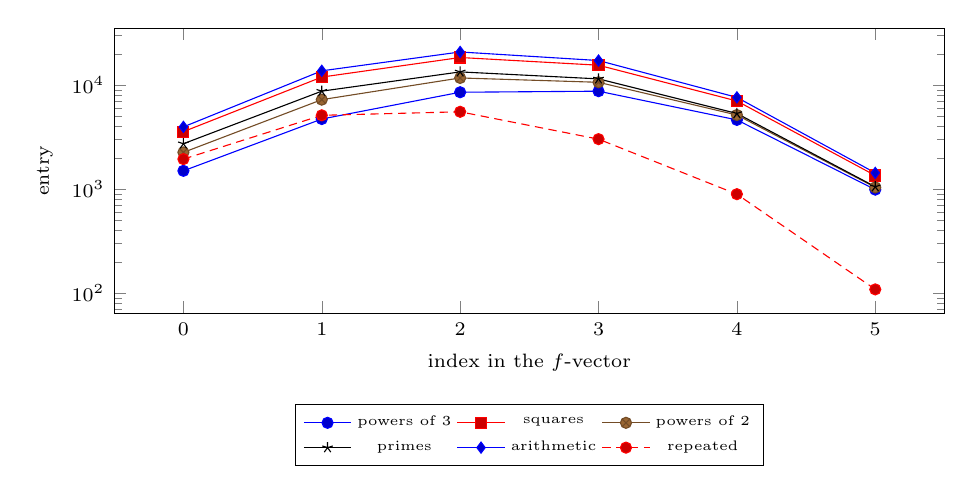
\begin{tikzpicture}
\begin{axis}[width=\linewidth, height=5.2cm, ymode=log, xlabel={index in the $f$-vector},
ylabel={entry}, legend style={font=\tiny, at={(0.5,-0.32)}, anchor=north, legend columns=3},
xtick={0,1,2,3,4,5}, tick label style={font=\scriptsize}, label style={font=\scriptsize}]
% BEGIN GENERATED fig-fvec
\addplot coordinates {(0,1506) (1,4744) (2,8586) (3,8787) (4,4652) (5,993)};
\addlegendentry{powers of 3}
\addplot coordinates {(0,3586) (1,12012) (2,18531) (3,15625) (4,7072) (5,1357)};
\addlegendentry{squares}
\addplot coordinates {(0,2266) (1,7285) (2,11782) (3,10702) (4,5185) (5,1044)};
\addlegendentry{powers of 2}
\addplot coordinates {(0,2745) (1,8795) (2,13472) (3,11540) (4,5365) (5,1059)};
\addlegendentry{primes}
\addplot coordinates {(0,3985) (1,13796) (2,20950) (3,17331) (4,7663) (5,1438)};
\addlegendentry{arithmetic}
\addplot coordinates {(0,1953) (1,5151) (2,5569) (3,3039) (4,898) (5,109)};
\addlegendentry{repeated}
% END GENERATED fig-fvec
\end{axis}
\end{tikzpicture}
\end{minipage}\hfill
\begin{minipage}{0.49\textwidth}\centering
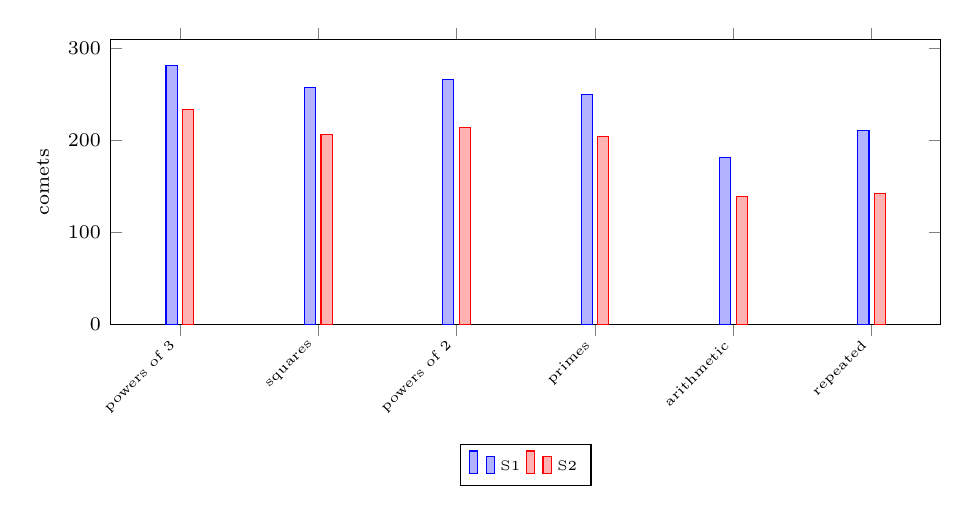
\begin{tikzpicture}
\begin{axis}[ybar, width=\linewidth, height=5.2cm, ylabel={comets},
symbolic x coords={%
% BEGIN GENERATED fig-comets-names
powers of 3,squares,powers of 2,primes,arithmetic,repeated
% END GENERATED fig-comets-names
}, xtick=data, x tick label style={rotate=45, anchor=east, font=\tiny},
tick label style={font=\scriptsize}, label style={font=\scriptsize}, bar width=4pt,
legend style={font=\tiny, at={(0.5,-0.42)}, anchor=north, legend columns=2},
enlarge x limits=0.1, ymin=0]
\addplot coordinates {
% BEGIN GENERATED fig-comets-s1
(powers of 3,281) (squares,257) (powers of 2,266) (primes,250) (arithmetic,181) (repeated,211)
% END GENERATED fig-comets-s1
};
\addplot coordinates {
% BEGIN GENERATED fig-comets-s2
(powers of 3,233) (squares,206) (powers of 2,214) (primes,204) (arithmetic,139) (repeated,142)
% END GENERATED fig-comets-s2
};
\legend{S1, S2}
\end{axis}
\end{tikzpicture}
\end{minipage}
\caption{Left: $f$-vector profiles (entries on a logarithmic scale) of the six S1 cells at $n=5$,
one curve per valuation family. Right: comet counts of systems S1 and S2 by valuation family at
$n=5$. Both panels are generated from the stored artifacts of Tables~\ref{tab:n5}.}\label{fig:profiles}
\end{figure}

\subsection{Every comet decided exactly (EXP-007)}\label{sec:exact}

On the failing controls the heuristic of the screening returns neither certificate,
so those cells read ``no certificate'' rather than ``not pointed''. The exact decision of
Algorithm~\ref{alg:lp} closes that gap: a cone is pointed exactly when \eqref{eq:feas} is
infeasible, and both outcomes carry a certificate re-verified by exact substitution outside the decider.

All sixteen cells are decided in 33 seconds total, with zero
certificate-verification failures\MV. Every comet certified pointed by the screening is
confirmed (no flips), and each failing control has exactly one comet that is
provably \emph{unpointed}: at $n=5$ the arithmetic valuations $(0,1,2,3,4)$ (180 pointed,
one unpointed) and the repeated valuations, and at $n=4$ the equal valuations. The data
therefore confirm, rather than merely agree with, the
failure of arithmetic valuations reported in \cite{JL25}, and localise it to a
single component out of 181\MV.

The logical direction matters: pointedness of every comet is a
\emph{sufficient} condition for dimension zero, so an unpointed comet proves
only that this certificate route does not close, never that finiteness fails. The
prevariety over-approximates the tropical variety\Dm.

Figure~\ref{fig:gens} gives the size of the nine unpointed comets, counted as the number of recession
generators in the stored certificates. The three S1 comets have \numGenSoneMin\ to \numGenSoneMax\ generators and the six S2 comets
\numGenStwoMin\ to \numGenStwoMax; the S2 cell at repeated valuations, the one whose $f$-vector has nine
entries (Table~\ref{tab:f5}), carries by far the largest comet, 2224 generators against 401 for the next. The figure shows only the size of the
failing component and not why it fails; the reason is the exact combination of generators stored in each
certificate, whose combination has between \numCertNzMin\ and \numCertNzMax\ nonzero coefficients: a small subset of the
generators already has a vanishing nonnegative combination, even in the comet of 2224 generators\MV.

\begin{figure}[t]\centering
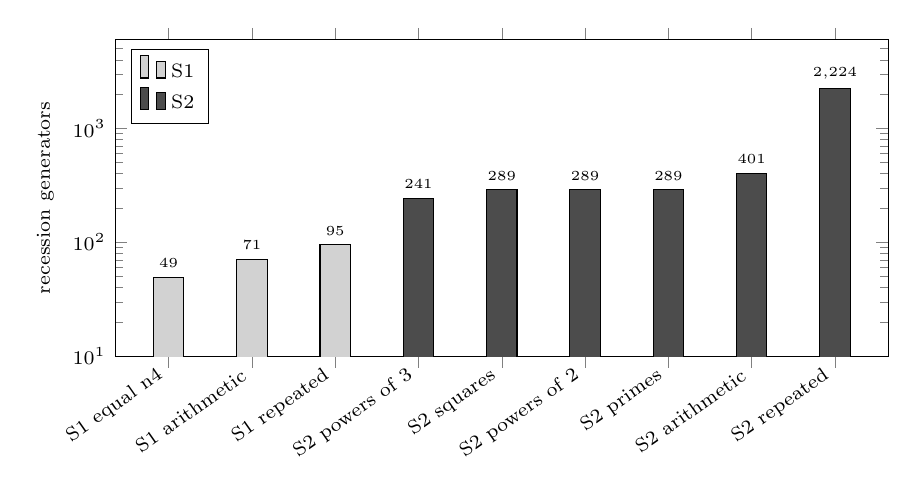
\begin{tikzpicture}
\begin{axis}[ybar, ymode=log, width=0.94\linewidth, height=5.6cm, ylabel={recession generators},
symbolic x coords={%
% BEGIN GENERATED fig-gens-names
S1 equal n4,S1 arithmetic,S1 repeated,S2 powers of 3,S2 squares,S2 powers of 2,S2 primes,S2 arithmetic,S2 repeated
% END GENERATED fig-gens-names
}, xtick={%
% BEGIN GENERATED fig-gens-names
S1 equal n4,S1 arithmetic,S1 repeated,S2 powers of 3,S2 squares,S2 powers of 2,S2 primes,S2 arithmetic,S2 repeated
% END GENERATED fig-gens-names
}, x tick label style={rotate=35, anchor=east, font=\scriptsize},
tick label style={font=\scriptsize}, label style={font=\scriptsize}, bar width=11pt,
legend style={font=\scriptsize, at={(0.02,0.97)}, anchor=north west},
enlarge x limits=0.08, ymin=10, ymax=6000, point meta=explicit, nodes near coords, nodes near coords style={font=\tiny}]
\addplot[fill=gray!35, bar shift=0pt] coordinates {
% BEGIN GENERATED fig-gens-s1
(S1 equal n4,49) [49] (S1 arithmetic,71) [71] (S1 repeated,95) [95]
% END GENERATED fig-gens-s1
};
\addplot[fill=black!70, bar shift=0pt] coordinates {
% BEGIN GENERATED fig-gens-s2
(S2 powers of 3,241) [241] (S2 squares,289) [289] (S2 powers of 2,289) [289] (S2 primes,289) [289] (S2 arithmetic,401) [401] (S2 repeated,2224) [2224]
% END GENERATED fig-gens-s2
};
\legend{S1, S2}
\end{axis}
\end{tikzpicture}
\caption{Recession generators of the single unpointed comet in each of the nine failing cells, on a
logarithmic scale: the equal-valuation cell at $n=4$ and two $n=5$ cells of system S1, and the six $n=5$ cells of
system S2. Counts are read from the stored exact certificates of the pointedness decision.}\label{fig:gens}
\end{figure}

The exact decision costs little next to the polyhedral computation. Figure~\ref{fig:times} plots, for the twelve $n=5$ cells, the
decider time against the \texttt{gfan} wall time of the same cell: the decider takes between \numRatioMin\ and
\numRatioMax\ percent of the \texttt{gfan} time. The comparison is of wall-clock seconds only; the \texttt{gfan} runs
used 30 threads (Algorithm~\ref{alg:gfan}) and the thread count of the decider is not recorded in its summary file. The figure does not show how the
decider scales with the number of generators beyond the largest comet of the grid, 2224 generators, which took 15.8 seconds.

\begin{figure}[t]\centering
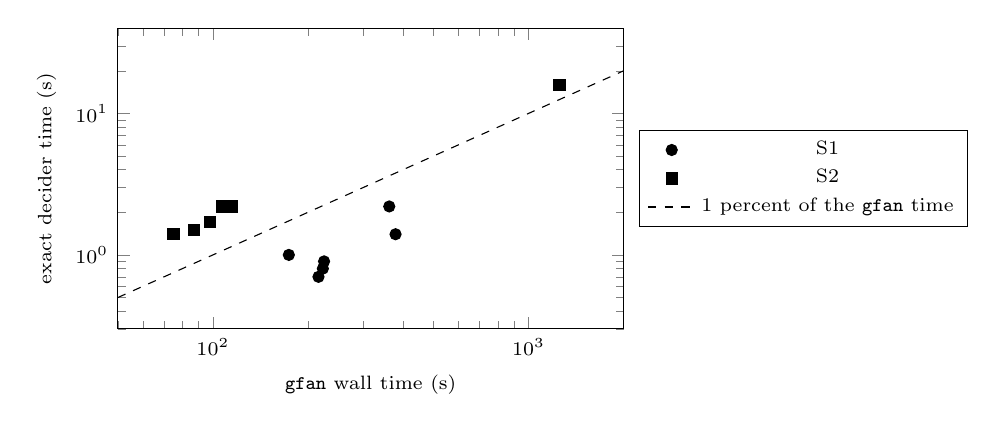
\begin{tikzpicture}
\begin{axis}[xmode=log, ymode=log, width=0.66\linewidth, height=5.4cm,
xlabel={\texttt{gfan} wall time (s)}, ylabel={exact decider time (s)},
legend style={font=\scriptsize, at={(1.03,0.5)}, anchor=west},
tick label style={font=\scriptsize}, label style={font=\scriptsize}, xmin=50, xmax=2000, ymin=0.3, ymax=40]
\addplot[only marks, mark=*] coordinates {
% BEGIN GENERATED fig-times-s1
(225,0.9) (362,2.2) (216,0.7) (223,0.8) (379,1.4) (174,1.0)
% END GENERATED fig-times-s1
};
\addplot[only marks, mark=square*] coordinates {
% BEGIN GENERATED fig-times-s2
(87,1.5) (115,2.2) (98,1.7) (75,1.4) (107,2.2) (1253,15.8)
% END GENERATED fig-times-s2
};
\addplot[dashed, no marks, domain=50:2000] {0.01*x};
\legend{S1, S2, 1 percent of the \texttt{gfan} time}
\end{axis}
\end{tikzpicture}
\caption{Exact decider time against \texttt{gfan} wall time for the twelve $n=5$ cells of Table~\ref{tab:n5}, both
on logarithmic axes; circles are system S1 and squares system S2, the dashed line marks one percent of the
\texttt{gfan} time. Times are read from the stored screening table and decision summary.}\label{fig:times}
\end{figure}


\subsection{Adding equations: what helps and what does not (EXP-008)}

Since removing the redundant symmetric equations is catastrophic, the converse is
worth measuring. At $n=4$, where the planar stratum \emph{is} the Dziobek stratum
and Dziobek's equations are therefore available (they are what
Hampton--Moeckel~\cite{HM06} needed when the Albouy--Chenciner equations alone
defeated their method), we ran the baseline against three enrichments: the energy--inertia
relation $e_{IU}$ (system A2), Dziobek's equations (A3) and both (A4). Table~\ref{tab:enrich} lists the
twelve cells; every comet is decided exactly, and the baseline cells reproduce the
$f$-vectors of Table~\ref{tab:n4} at all three shared valuations.

\begin{table}[t]\centering\footnotesize\setlength{\tabcolsep}{3pt}
% BEGIN GENERATED table-enrich
\begin{tabular}{@{}llrrrrl@{}}
\toprule
Valuations & System & comets & pointed & unpointed & gfan (s) & $f$-vector \\
\midrule
$(0,0,0,0)$ equal & A1, baseline & 1 & 0 & 1 & 13.2 & \texttt{1 49 66 18} \\
$(0,0,0,0)$ equal & A2, $+\,e_{IU}$ & 1 & 0 & 1 & 17.9 & \texttt{1 49 66 18} \\
$(0,0,0,0)$ equal & A3, $+$ Dziobek & 1 & 0 & 1 & 17.6 & \texttt{1 37 48 12} \\
$(0,0,0,0)$ equal & A4, $+$ both & 1 & 0 & 1 & 17.1 & \texttt{1 37 48 12} \\
\midrule
$(1,2,4,8)$ powers of 2 & A1, baseline & 10 & 10 & 0 & -- & \texttt{63 119 82 19} \\
$(1,2,4,8)$ powers of 2 & A2, $+\,e_{IU}$ & 10 & 10 & 0 & -- & \texttt{63 119 82 19} \\
$(1,2,4,8)$ powers of 2 & A3, $+$ Dziobek & 7 & 7 & 0 & -- & \texttt{64 131 101 27} \\
$(1,2,4,8)$ powers of 2 & A4, $+$ both & 7 & 7 & 0 & -- & \texttt{64 131 101 27} \\
\midrule
$(0,1,2,3)$ arithmetic & A1, baseline & 9 & 9 & 0 & 66.3 & \texttt{83 164 108 23} \\
$(0,1,2,3)$ arithmetic & A2, $+\,e_{IU}$ & 9 & 9 & 0 & 92.2 & \texttt{82 162 107 23} \\
$(0,1,2,3)$ arithmetic & A3, $+$ Dziobek & 6 & 6 & 0 & 71.5 & \texttt{86 183 135 34} \\
$(0,1,2,3)$ arithmetic & A4, $+$ both & 6 & 6 & 0 & 80.6 & \texttt{85 181 134 34} \\
\bottomrule
\end{tabular}
% END GENERATED table-enrich
\caption{The enrichment grid at $n=4$ (twelve cells; all runs in arbitrary precision). Every comet is
decided exactly. The \texttt{gfan} seconds are those stored in \texttt{table.json} of the experiment;
the powers-of-two cells are read from the stored \texttt{gfan} outputs and their wall times are
not stored (marked ``--'').}\label{tab:enrich}
\end{table}

Two results run against intuition. First, adding equations does not always shrink the
$f$-vector: at equal valuations it shrinks, with the entries falling from $(49,66,18)$ to
$(37,48,12)$ (reductions of 24, 27 and 33 percent), but it \emph{grows} it at powers of two
(entries $119,82,19$ to $131,101,27$) and at arithmetic valuations ($164,108,23$ to $183,135,34$)\MV.
The prevariety as a set
must not be confused with the subdivision that represents it:
intersecting more tropical hypersurfaces can only shrink the set while refining the
fan, so cone counts may rise\Dm. The invariant that behaves monotonically in our data
is the comet count, which falls from 10 to 7 and from 9 to 6 when Dziobek is
adjoined (Figure~\ref{fig:enrich}). Second, Dziobek's equations do not rescue the hard equal-valuation case: the
prevariety entries fall as above and its
single comet stays provably unpointed. The enrichment that rescued the
\emph{algebraic} proof therefore does not rescue the \emph{tropical} certificate at
the same specialisation, which separates two roles that are easy to conflate. The cells with Dziobek
cover the planar noncollinear stratum only (the collinear classes are classical); the positive cells of
A3 and A4 are not claimed as full certificates, since the A1 cells already provide those.

\begin{figure}[t]\centering
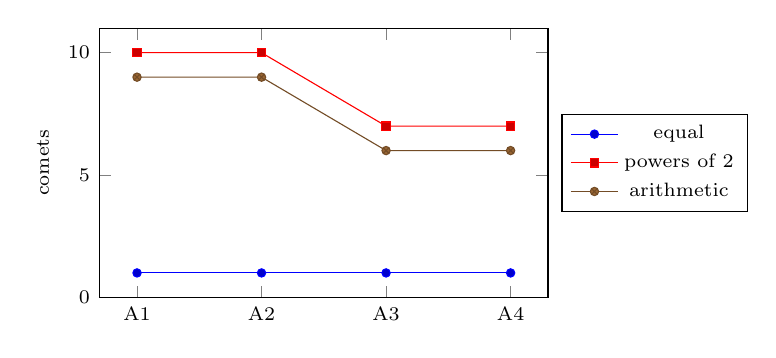
\begin{tikzpicture}
\begin{axis}[width=0.6\linewidth, height=5cm, ylabel={comets}, symbolic x coords={A1,A2,A3,A4},
xtick=data, legend style={font=\scriptsize, at={(1.03,0.5)}, anchor=west},
tick label style={font=\scriptsize}, label style={font=\scriptsize}, ymin=0, ymax=11, mark size=1.5pt]
% BEGIN GENERATED fig-enrich
\addplot coordinates {(A1,1) (A2,1) (A3,1) (A4,1)};
\addlegendentry{equal}
\addplot coordinates {(A1,10) (A2,10) (A3,7) (A4,7)};
\addlegendentry{powers of 2}
\addplot coordinates {(A1,9) (A2,9) (A3,6) (A4,6)};
\addlegendentry{arithmetic}
% END GENERATED fig-enrich
\end{axis}
\end{tikzpicture}
\caption{Comet count along the enrichment ($\mathrm{A1}$ baseline, $\mathrm{A2}$ with the
energy--inertia relation, $\mathrm{A3}$ with Dziobek's equations, $\mathrm{A4}$ with both) at the
three $n=4$ valuations, generated from Table~\ref{tab:enrich}.}\label{fig:enrich}
\end{figure}

By contrast the energy--inertia relation is tropically inert: it reproduces the
baseline $f$-vector exactly at two of the three valuations (equal and powers of two) and shrinks it slightly
at the arithmetic one ($82,162,107,23$ against $83,164,108,23$). Dependence in the ideal
predicts tropical relevance in neither direction, which is the sharper form of the
lesson above, and it lets us drop that equation from expensive runs at no cost\MV.

\section{Bit-width provenance and what the certificates rest on}\label{sec:validation}

The word \emph{certified} in the screening and reproduction sections applies to the exact decisions
on comets, not to the polyhedral computation. Table~\ref{tab:bits} states which arithmetic mode produced
which result.

\begin{table}[t]\centering\footnotesize
\begin{tabular}{@{}L{3.6cm}L{3.4cm}L{5.4cm}@{}}
\toprule
Experiment & \texttt{gfan} arithmetic & Result that rests on it \\
\midrule
EXP-003 ($n=5$, two valuations) & \texttt{-{}-bits 64} (fast path) & $f$-vectors of \cite{JL25}, pointed cone for powers of 3 \\
EXP-004 ($n=4,5$, 16 cells) & \texttt{-{}-bits 64} & Tables~\ref{tab:n5} and \ref{tab:n4}, working families, S2 failure \\
EXP-008 ($n=4$, 12 cells) & \texttt{-{}-bits 0} (arbitrary precision) & Table~\ref{tab:enrich} \\
EXP-005 ($n=6$, 0.7) & \texttt{-{}-bits 64}; arbitrary precision & overflow abort; internal assertion \\
\bottomrule
\end{tabular}
\caption{Arithmetic mode of the prevariety runs.}\label{tab:bits}
\end{table}

The overflow-checked rerun of the $n=5$ computation that \cite{JL25} describe (about ten times slower) was
not repeated, and the full arbitrary-precision rerun of the positive $n=5$ cells was queued as hardening
and no record shows that it ran. The $n=5$ certificates therefore rest on the fast path alone\Dm. Two facts
bound the risk: on the fast path an arithmetic overflow is detected and aborts the run, so a silent wrong
answer is not the failure mode (the $n=6$ attempts of Section~\ref{sec:six} aborted in exactly this way)\Dm;
and the arbitrary-precision run of the enrichment grid reproduces the $n=4$ $f$-vectors of the fast-path
screening exactly at the three shared valuations, $(1,49,66,18)$, $(63,119,82,19)$ and $(83,164,108,23)$\MV.
That agreement is a partial validation at $n=4$ only. The arbitrary-precision rerun of the $n=5$
positive cells is an open item (Section~\ref{sec:limits}).

\section{Censuses across two independent engines (EXP-006)}\label{sec:census}

Two of the $n=3$ censuses do not finish within a 900-second limit in our own engine. % voice-ok
We recomputed them with msolve (Gr\"obner bases, rational univariate representation and
certified real-root isolation), keeping our exact machinery as the verification
layer: msolve returns rational isolating boxes, and containment of an exact
algebraic point in a rational box is decided exactly. Both open cells close in under
a second each, and for all four mass vectors the positive census is exactly the
classical answer, one equilateral point and one collinear point per ordering, with
every one of our independently computed exact points inside a distinct box and no
unexplained boxes\MV. Two implementations that share no code agree on every decided
instance.

The same computation shows that the enriched planar $n=4$ system does not admit an
isolated census to compare with the published equal-mass class count (a numerical census of Sim\'o \cite{Simo78}\Um,
the symmetric configurations of four equal masses of Albouy \cite{Albouy96}\Um\ and the rigorous counts of
\cite{MZ19}): msolve reports
the affine system to have dimension one, so there is no
isolated census to compare\MV. Diagnostics exclude the vanishing-distance loci as the
cause, which leaves the reading the literature already acts on: the census belongs in
the torus, where all mutual distances are invertible, which is precisely the setting
of~\cite{HM06}\Dm. We record the count as untested rather than quoting the published
value as if we had reproduced it.

Following that lesson, we attempted the $n=4$ equal-mass census where it belongs,
in the torus, by two independent exact formulations: the enriched planar system
under a Rabinowitsch saturation of the distance product (seven unknowns) and the
z-system of~\cite{HM06} (twelve unknowns, the mutual distances joined by the
Dziobek variables). The exact square of Section~\ref{sec:calib} satisfies the first system,
checked by exact residual substitution\MV. Neither formulation produced any
msolve output within a mechanically enforced time limit of 3600 seconds % voice-ok
per route (EXP-009), so the published equal-mass counts remain untested by us.
We note that the literature contains, to our knowledge, no direct algebraic
solve of this census either\Um: \cite{HM06} bound the count by a mixed volume
rather than solving, and the rigorous equal-mass counts of~\cite{MZ19} come from
interval methods. The measured cliff between $n=3$ (both censuses close in under
a second) and $n=4$ (no output in an hour, twice) points counting towards bounds
rather than solutions, and finiteness towards dimension computations, as follows.

\medskip
\noindent\textbf{Dimension of the $n=4$ Dziobek variety (EXP-010).}
The object is the Dziobek variety of $n=4$ (Dziobek \cite{Dziobek00}; bibliographic data only): the vanishing of the cleared Dziobek
differences
\begin{equation}\label{eq:dziobek}
S_{12}S_{34}=S_{13}S_{24}=S_{14}S_{23}
\end{equation}
together with the planar
Cayley--Menger determinant, in the torus of the six mutual distances. Masses do
not appear in this formulation, and generic finiteness corresponds to this
variety having the dimension of the projectivized mass space, three. The
instrument keeps every algebraic call zero-dimensional by construction: recorded
random integer linear sections of codimension three (which should meet the
variety in finitely many points, whose number is degree data) and codimension
four (which should miss it), decided by msolve under caps, with a deterministic
Gr\"obner staircase computation run separately. A validation test discriminates
three exact anchors in one second: the exact square of Section~\ref{sec:calib} lies on the
variety (certified by polynomial reduction modulo $8a^3=4+\sqrt{2}$ written as
two polynomial relations, no radical heuristics), the unit tetrahedron satisfies
the Dziobek equations but is excluded by Cayley--Menger, and the $3$-$4$-$5$
rectangle satisfies Cayley--Menger but violates the Dziobek equations\MV.

The probes show an asymmetry that is itself the finding. Two independent
codimension-four random sections
(coefficients drawn uniformly from $[-10^6,10^6]$ by a seeded generator, the
draws archived verbatim) came back \emph{empty} in one second each (msolve's
dimension $-1$ output), which is probabilistic-exact support for the Dziobek
variety having dimension at most three, exactly the value the generic
finiteness picture predicts and exactly the direction such arguments consume
(what must be excluded is excess dimension)\MV. By contrast, both
codimension-three census probes and a deterministic Gr\"obner staircase
computation did not finish within their time limits (900 and 1800 seconds), so
no degree data and no dimension lower bound beyond the exact witness were
produced, and the census half of the instrument is not pursued at this size. Since only an a-priori degree ceiling is
available (B\'ezout with the stripped degrees $9\cdot 9\cdot 6 = 486$), the
emptiness result carries a failure estimate of order $10^{-3}$ per draw; it is
evidence, not proof\Dm. For the upper-bound direction the natural tools are cheap
emptiness probes and the partial-Gr\"obner device of Dias--Pan~\cite{DP18}
(dimension bounds from the union of leading monomials of tractable subideal
bases); certified witness sets serve the lower-bound direction. The next case is
the spatial five-body Dziobek variety, following the proof shape of~\cite{DP18}
with exact instruments.

\medskip
\noindent\textbf{The scaling test at $n=5$ (EXP-011).} At $n=5$ the same
instruments meet a computational wall. The object is the fifteen cleared Dziobek
product differences over all quadruples of five bodies together with the spatial
Cayley--Menger equation, in the torus of the ten mutual distances; the cut is an
overvariety of the spatial Dziobek central configurations (degenerate strata
satisfy the products trivially, as an exact point of the validation set shows:
the unit-side, unit-slant bipyramid with $r_{45}^2 = 8/3$, whose membership
reduces to rational arithmetic). The three-anchor validation passed in four
seconds; every msolve section probe, including the codimension-five emptiness
probes that cost one second at $n=4$, capped at 300 seconds; and a run of the
partial-Gr\"obner instrument (fifteen subideals, each one product plus
Cayley--Menger plus the saturation, 120 seconds apiece under sympy) completed
a single subideal, leaving a vacuous union bound\MV. Nothing refuted the expected
dimension four; nothing supported it either. We read the wall as an engine
fact rather than a mathematical one: \cite{DP18} report completing the
identical leading-term pattern on an eleven-variable system in minutes under
Singular, which motivates a change of Gr\"obner engine\Vm.

\medskip
\noindent\textbf{Engine comparison and the $n=5$ dimension (EXP-012, EXP-013,
EXP-014).} Three further computations settle the engine question and reduce the
$n=5$ question to a single open decision. First, the wall is an engine effect:
Singular over $\mathbb{Q}$ (release and binary hash in Table~\ref{tab:tools}) completes twelve of
the identical fifteen subideal jobs at 0.4--1 seconds each, against one completion
near 100 seconds under sympy\MV\ (Figure~\ref{fig:singular}). An exact-reproduction control also shows that
sympy's Gr\"obner output uses lexicographic ordering whatever order is requested,
so the leading terms harvested in the EXP-011 run were lex leads of grevlex
elements; that harvest gave only a vacuous bound, and no result depends on it.
msolve's basis mode is modular, so it is used for screening only: an unlucky
prime can enlarge a leading ideal and fake a \emph{lower} dimension bound.
Second, the union bound gives dimension at most 5, and the fifteen-product
system without Cayley--Menger terminates completely in nine seconds, so its
staircase dimension is the true Krull dimension: \emph{exactly} 5, matching the
rank-one parametrization count\MV. The cost law is sharp: every computation
without Cayley--Menger runs in seconds, every mix of the products with
Cayley--Menger caps. Third, the incremental extension of the completed
products basis by Cayley--Menger (whose normal form against that basis is
nonzero, so the cut is a proper subvariety) also did not terminate within
1800 seconds. The results for the spatial five-body Dziobek cut
are therefore: products variety of dimension exactly 5, cut of dimension at
most 5, expected value 4 undecided. The remaining decision (does Cayley--Menger
vanish identically on a top component?) calls for certified witness sets, and
the cost law, measured twice, guides the work on the symmetric strata below.

\begin{figure}[t]\centering
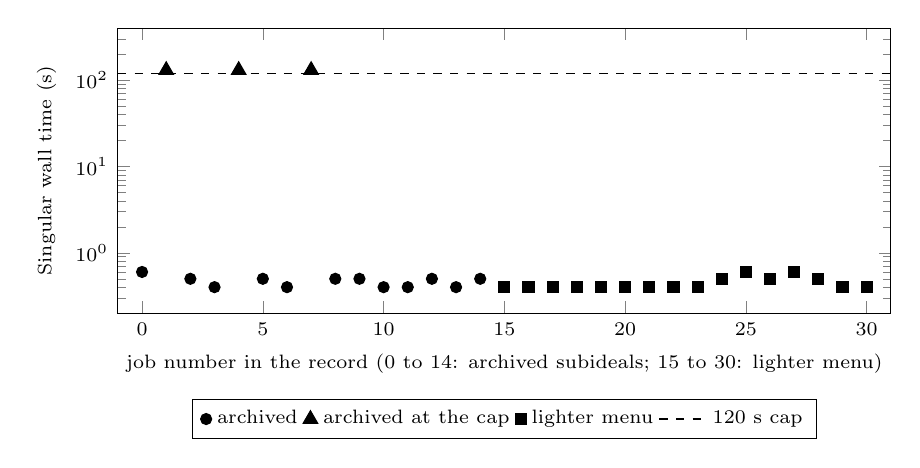
\begin{tikzpicture}
\begin{axis}[ymode=log, width=0.94\linewidth, height=5.2cm,
xlabel={job number in the record (0 to 14: archived subideals; 15 to 30: lighter menu)},
ylabel={Singular wall time (s)}, ymin=0.2, ymax=400, xmin=-1, xmax=31,
legend style={font=\scriptsize, at={(0.5,-0.3)}, anchor=north, legend columns=4},
tick label style={font=\scriptsize}, label style={font=\scriptsize}]
\addplot[only marks, mark=*] coordinates {
% BEGIN GENERATED fig-singular-done
(0,0.6) (2,0.5) (3,0.4) (5,0.5) (6,0.4) (8,0.5) (9,0.5) (10,0.4) (11,0.4) (12,0.5) (13,0.4) (14,0.5)
% END GENERATED fig-singular-done
};
\addplot[only marks, mark=triangle*, mark size=3pt] coordinates {
% BEGIN GENERATED fig-singular-capped
(1,130.7) (4,130.7) (7,130.8)
% END GENERATED fig-singular-capped
};
\addplot[only marks, mark=square*] coordinates {
% BEGIN GENERATED fig-singular-menu
(15,0.4) (16,0.4) (17,0.4) (18,0.4) (19,0.4) (20,0.4) (21,0.4) (22,0.4) (23,0.4) (24,0.5) (25,0.6) (26,0.5) (27,0.6) (28,0.5) (29,0.4) (30,0.4)
% END GENERATED fig-singular-menu
};
\addplot[dashed, no marks, domain=-1:31] {120};
\legend{archived, archived at the cap, lighter menu, 120 s cap}
\end{axis}
\end{tikzpicture}
\caption{Wall time of the 31 Singular jobs of the partial Gr\"obner spike on a logarithmic scale: the 15 archived
subideals of the spatial Dziobek cut (twelve complete, three reach the 120 s cap) and the 16 jobs of the lighter
menu, all complete. Times are read from the stored timing file; the capped readings exceed 120 s by the
overhead of the time limit.}\label{fig:singular}
\end{figure}

The figure shows the sharp separation behind that reading: all 28 completed jobs take between \numSingMin\ and \numSingMax\
seconds, and the three archived subideals that do not complete (jobs 1, 4 and 7, which share the body pair $\{1,2\}$
in their pairing structure) hit the cap. No job takes an intermediate time, so the cost is a threshold effect of the
subideal and not a smooth function of its size; the figure cannot say what the threshold is, and the records leave it unexplained.

\section{The two-pair symmetric stratum of six bodies (EXP-015 to EXP-023)}\label{sec:stratum}

Dias--Pan~\cite{DP18} proved generic finiteness for the \emph{cross} symmetric
class of the planar six-body problem (four bodies on the reflection axis, one
mirror pair)\Vm. We study the neighbouring class, with two bodies on the axis
and \emph{two} mirror pairs. A targeted search found no published
finiteness result for this class; no MathSciNet or zbMATH search was made\Um.
This section states what is proved, by what argument, and what is open, under the claim rule
of the Introduction. The result is a status report: no finiteness statement is claimed for the stratum.

\subsection{The object and its reduction}

Bodies 1 and 2 sit on the axis at $(0,a_1)$ and $(0,a_2)$; pair A is $(\pm u,v)$ and pair B is
$(\pm p,q)$, with $u,p>0$. The gauge fixes translation and scale, $a_1=1$, $a_2=-1$. The open stratum
$\mathcal S$ consists of collision-free configurations with distinct pair heights, $f:=v-q\ne0$. The
exact quotient derivation gives nine distance variables
($r_{12}$; $d_{1A},d_{1B},d_{2A},d_{2B}$; $w_A=2u$, $w_B=2p$; $c_s=r_{35}$, $c_x=r_{36}$)\MV\ and the
relation
\begin{equation}\label{eq:cxcs}
c_x^2-c_s^2=w_A\,w_B ,
\end{equation}
from $(u+p)^2-(u-p)^2=4up$\MV. With all six masses free the Laura--Andoyer equations of the two pairs evaluate
exactly to
\begin{equation}\label{eq:pair}
L_{34}=-2u\,(m_5-m_6)(q-v)\,\frac{c_x^3-c_s^3}{c_s^3c_x^3},\qquad
L_{56}=+2p\,(m_3-m_4)(q-v)\,\frac{c_x^3-c_s^3}{c_s^3c_x^3} .
\end{equation}
The identities \eqref{eq:pair} are machine-verified\MV. On $\mathcal S$ one has $q\ne v$, $u,p\ne0$ and, by \eqref{eq:cxcs}, $c_x\ne c_s$, so $L_{34}=L_{56}=0$ forces
$m_5=m_6$ and $m_3=m_4$: the masses within each pair are equal (the pair-equality statement)\Dm. The
factorization \eqref{eq:pair} is a machine identity; the consequence is its immediate reading. The
statement is limited to $q\ne v$: on the sub-stratum $q=v$ both equations vanish identically and force
nothing, so that sub-stratum is outside the scope. An attack-based review of the claims records the
pair-equality statement as \emph{not tested}: the informative attack, which keeps independent masses on all
four pair bodies, lets the geometry vary and solves ten equations in ten unknowns, was not run, and
an earlier attack that varied $m_A$ against $m_B$ tested a proposition nobody made
(\texttt{CC/context/2026-08-25-adversarial-audit.md}, sections 5 and 6). % voice-ok
No lemma environment is used for the pair-equality statement for that reason.

By the reflection $(34)(56)$, which preserves all distances and reverses orientation, $L_{12},L_{34},L_{56}$
vanish and the other twelve equations pair up with signs, leaving six independent equations
$\{L_{13},L_{15},L_{23},L_{25},L_{35},L_{36}\}$, each linear in $(m_1,m_2,m_A,m_B)$\Dm; the pairing is
confirmed at a witness geometry, where the six partner equations are exact negatives of the block
equations\MV. The block is a $6\times4$ matrix $J(u,v,p,q)$ whose kernel gives the admissible masses,
\begin{equation}\label{eq:kernel}
J(u,v,p,q)\begin{pmatrix}m_1\\ m_2\\ m_A\\ m_B\end{pmatrix}=0,\qquad
J=\bigl(J[L][c]\bigr)_{\,L\in\{L_{13},L_{15},L_{23},L_{25},L_{35},L_{36}\},\ c\in\{m_1,m_2,m_A,m_B\}},
\end{equation}
where $J[L][c]$ is the coefficient of the mass $c$ in the equation $L$\Dm\ (\path{CC/context/2026-08-20-stratum-theorem-assembly.md}, section~1). % voice-ok
The gauged shape variety $X$ has dimension 4 (five ungauged), by two engines in one second each\MV.
Its closure $X^{+}$ of the image of the irreducible parameter space $(a_1,a_2,u,v,p,q)$ is
irreducible of dimension 4\Dm. The matrix has rank 4 at the two exact witnesses
$W_1=(a_1,a_2,u,v,p,q)=(3,-1,2,1,1,-2)$ and $W_2=(2,-2,1,2,3,-1)$\MV. The equal-mass regular hexagon lies in
the stratum through the block (all six equations vanish exactly), and its dihedral symmetry lowers the
rank to exactly 3 (a nonzero $3\times3$ minor of value $147/128-735\sqrt3/512$, all $4\times4$ minors
zero)\MV. The complete catalogue of the $2\times2$ minors, computed with the inverse-cube differences
$s(a,b)=a^{-3}-b^{-3}$ as abstract symbols, has 84 nonzero entries of the 90 possible, a count reproduced
by an independent count over six random shapes\MV.

\subsection{The fibre-dimension count}

Let $R_j=\{\operatorname{rank}J\le j\}\cap X^{+}$ and $I=\{(x,m):x\in X^{+},\ m\in\ker J(x),\ m\ne0\}$ with
projection $\pi:I\to\mathbb{R}^4$ to mass space. Over the locus of rank exactly $r$ the fibre of $I\to X^{+}$ is
the kernel, of dimension $4-r$, so
\begin{equation}\label{eq:count}
\dim I=\max_{r}\bigl[\dim\{\operatorname{rank}J=r\}+(4-r)\bigr].
\end{equation}

\begin{proposition}\label{prop:count}
If $\dim R_0\le0$, $\dim R_1\le1$, $\dim R_2\le2$ and $R_3\ne X^{+}$, then $\dim I\le4$.
\end{proposition}
\begin{proof}
Term by term in \eqref{eq:count}: for $r=4$ the term is at most $4+0$; for $r=3$, irreducibility of $X^{+}$ and
$R_3\ne X^{+}$ give $\dim R_3\le3$, so the term is at most $3+1$; for $r=2$ it is at most $2+2$, for $r=1$ at
most $1+3$ and for $r=0$ at most $0+4$.
\end{proof}

From $\dim I\le 4=\dim\mathbb{R}^4$ the projection $\pi$ has finite generic fibres, or is not dominant, in which
case generic masses admit no configuration of the stratum at all; this is the fibre-dimension argument of
the Dias--Pan pattern \cite{DP18} (the record's section~2 of
\path{CC/context/2026-08-20-stratum-theorem-assembly.md}, lines 26--62). % voice-ok
The four hypotheses are the \emph{ladder}. Following the case numbering of the records, case $k$ is the statement
$\dim R_{k-1}\le k-1$ (for $k=1,2,3$) and $R_3\ne X^{+}$ (for $k=4$). The centred pentagon below shows that
$\dim R_2=2$ is attained, so the bound for $k=3$ is sharp.

\subsection{The proved cases and their pointers}

\begin{table}[t]\centering\footnotesize
\begin{tabular}{@{}L{0.5cm}L{3.0cm}L{2.2cm}L{6.6cm}@{}}
\toprule
$k$ & Statement & Status & Written proof in the records \\
\midrule
0 & $R_0$ misses $\mathcal S$ & proved\Dm\MV & Lemma~\ref{lem:r0} below; \path{CC/experiments/EXP-022-collar-coverings/r0-lemma.py} (docstring) \\
1 & $\dim R_0\le 0$ & proved\Dm\MV & piece 5, \path{CC/context/2026-08-02-rank-floor-lemma-dossier.md} lines 199--236 \\ % voice-ok
2 & $\dim R_1\le 1$ & proved\Dm\MV & pieces 1 to 4, same file, lines 8--155 (Lemma~\ref{lem:piece1} gives piece 1) \\ % voice-ok
3 & $\dim R_2\le 2$ & reduced to four bilinear conditions\Dm & piece 7b, same file, lines 313--341; certified covering below \\ % voice-ok
4 & $R_3\ne X^{+}$ & proved\Dm\MV & Proposition~\ref{prop:k4} below; same file, lines 270--289 \\ % voice-ok
\bottomrule
\end{tabular}
\caption{Status of the cases of the ladder. A case is called proved only with a written proof in this paper
or at the cited lines.}\label{tab:cases}
\end{table}

\begin{lemma}[piece 1]\label{lem:piece1}
On $\mathcal S$ the $2\times2$ minor of $J$ on rows $\{L_{35},L_{36}\}$ and columns $\{m_1,m_2\}$ equals
\begin{equation}\label{eq:piece1}
M=s(d_{1A},d_{1B})\,s(d_{2A},d_{2B})\,\bigl(-2\,u\,p\,(v-q)(a_1-a_2)\bigr).
\end{equation}
Hence $\operatorname{rank}J\ge2$ on $\mathcal S$ outside $E=\{d_{1A}=d_{1B}\}\cup\{d_{2A}=d_{2B}\}$.
\end{lemma}
\begin{proof}
The four entries are single terms of the form $s(d_{iA},d_{iB})\,\Delta$, with the same $s$-factor in each column,
so the $s$-factors come out of the determinant. The polynomial bracket $\Delta_{351}\Delta_{362}-\Delta_{361}\Delta_{352}$
equals $-2up(v-q)(a_1-a_2)$ identically (an expanded residual that is the zero polynomial; by hand,
$\alpha\gamma-\beta\delta=-(v-q)(a_1-a_2)$ in the height variables). On $\mathcal S$ the bracket is nonzero because
$u,p>0$, $v\ne q$ and $a_1\ne a_2$. Where it is nonzero the minor is nonzero unless an $s$-factor vanishes,
which is the set $E$.
\end{proof}

\begin{lemma}[$k=0$]\label{lem:r0}
$R_0\cap\mathcal S=\emptyset$.
\end{lemma}
\begin{proof}
The entries $J[L_{23}][m_1]=s(r_{12},d_{1A})\,u\,e_{12}$ and $J[L_{13}][m_2]=-s(r_{12},d_{2A})\,u\,e_{12}$ (and the
analogous entries for pair B) are single $s$-terms with nonvanishing monomial brackets on $\mathcal S$. If $J=0$ then
$d_{1A}=d_{2A}=r_{12}=2$ and $d_{1B}=d_{2B}=2$. From $d_{1A}^2-d_{2A}^2=-4v$ one gets $v=0$, and likewise $q=0$,
so $f=v-q=0$, contradicting $q\ne v$ on $\mathcal S$.
\end{proof}

\begin{proposition}[$k=4$]\label{prop:k4}
$R_3\ne X^{+}$, hence $\dim R_3\le3$.
\end{proposition}
\begin{proof}
At $W_1$ the matrix has rank 4, by exact radical arithmetic, so some $4\times4$ minor $g_4$ satisfies $g_4(W_1)\ne0$
exactly. The point $W_1$ is a parametrized geometry, hence a point of $X^{+}$. On $R_3$ every $4\times4$ minor
vanishes, so $R_3\subset\{g_4=0\}\cap X^{+}$. Since $X^{+}$ is irreducible of dimension 4 and $g_4$ does not vanish
identically on it, Krull's principal ideal theorem gives $\dim(\{g_4=0\}\cap X^{+})=3$.
\end{proof}

The cases $k=1$ and $k=2$ combine closed-form minors with exact witnesses. Four minors of the catalogue factor into
monomials times products of the symbols $x_i=s(d_{iA},r_{12})$ and $y_i=s(d_{iB},r_{12})$; the Boolean analysis of
the four products shows that $\operatorname{rank}J<2$ forces $x_1x_2=y_1y_2=y_1x_2=x_1y_2=0$, hence one of two branches
($d_{1A}=d_{1B}=r_{12}$ or $d_{2A}=d_{2B}=r_{12}$), each of codimension two. On each branch the mixed-column minors
add a third condition drawn from five explicit degenerations, each proper because the 3-4-5 witness
$(a_1,a_2,u,v,p,q)=(5,0,3,4,4,-3)$ (and its mirror) lies on the branch and violates all five; whence
$\dim R_1\le1$ (piece 4). For $k=1$ the two height sub-branches are empty by one-line substitutions, and the remaining
cuts are proper by witnesses over $\mathbb{Q}(\sqrt3)$, giving $\dim R_0\le0$ (piece 5). Every identity is verified
exactly in the records, and the 84-minor catalogue is the input of the Boolean analysis. We do not reproduce those two
proofs here; Table~\ref{tab:cases} points to their lines, and the status of each is stated by that pointer.

\subsection{The case \texorpdfstring{$k=3$}{k=3}: reduced, not closed}

On the region where the corner minor $\{L_{13},L_{23}\}\times\{m_1,m_2\}$ is nonzero (off
$\{d_{1A}=r_{12}\}\cup\{d_{2A}=r_{12}\}$), the eight borders of that corner factor, with all four identities verified
exactly, and
$R_2$ lies in the common zero set of four equations, each with at most five $s$-monomial terms:
\begin{equation}\label{eq:bilinear}
b_{13}J[L_{15}][c]=b_{15}J[L_{13}][c],\qquad a_{23}J[L_{25}][c]=a_{25}J[L_{23}][c],\qquad c\in\{m_A,m_B\},
\end{equation}
where $a_{23}=s(r_{12},d_{1A})\,u\,e_{12}$, $b_{13}=-s(r_{12},d_{2A})\,u\,e_{12}$, $b_{15}=-s(r_{12},d_{2B})\,p\,e_{12}$ and
$a_{25}=s(r_{12},d_{1B})\,p\,e_{12}$ are the clean entries\MV. All four conditions are exactly nonzero at $W_1$, $W_2$ and the
hexagon, so by irreducibility and Krull each cuts $X^{+}$ in dimension 3, and $\dim R_2\le 3$ follows on the good region;
the case needs $\dim R_2\le2$, that is a second cut that is not identically zero on any 3-dimensional component of
the first, and that statement has no written proof in the records\Dm. The routes tried to close it are
the computational ones of Table~\ref{tab:stratum}: the single-minor Gr\"obner cuts (EXP-019), the sign-chamber relaxation
(EXP-020) and the certified covering (EXP-021, EXP-022). The covering does not prove the case by itself, because its
statement is not assembled (below).

The sign-chamber relaxation asks whether the eight conditions can hold together at rank at most two when only
their sign pattern is kept. Six of the conditions have three terms and two have five. The count runs over the 24 feasible orientation
chambers. Within each, the 22 ordering atoms of the inverse-cube differences $s(a,b)$ and up to four bracket atoms are left free
except for the forced sums, a sound superset of the real sign patterns, and an exact GF(2) inclusion--exclusion count (256
affine-system ranks per chamber) gives the number of surviving assignments. An empty residual in every chamber would have been a sound
emptiness conclusion. Figure~\ref{fig:chambers} shows the outcome: no chamber is empty, and the total is \numChamberTotal\ assignments.
Every count is one, two or four times \numChamberUnit, with twelve, eight and four chambers at those levels, so the
distribution is quantized and not concentrated in a few chambers; the four largest chambers hold 16 of the 44 units, 36 percent.
The figure counts a superset and says nothing about which assignments are geometric. The reason the relaxation fails
is the freedom it grants: an ordering atom is a function of the coordinates. The first coupling in closed form is
\begin{equation}\label{eq:coupling}
\operatorname{sign}s(d_{1A},w_A)=\operatorname{sign}\bigl(4u^2-d_{1A}^2\bigr)=\operatorname{sign}\bigl(3u^2-h_1^2\bigr),\qquad h_1=a_1-v,
\end{equation}
because $w_A=2u$, $s(a,b)>0$ exactly when $a<b$ and $d_{1A}^2=u^2+h_1^2$\Dm\ (\path{CC/experiments/EXP-020-chamber-enumeration/verdict.md}). % voice-ok
So this ordering atom is decided by comparing the height $|h_1|$ with $\sqrt3\,u$, an atom the free-atom count cannot see, and
the same holds for the other ordering atoms\Dm.

\begin{figure}[t]\centering
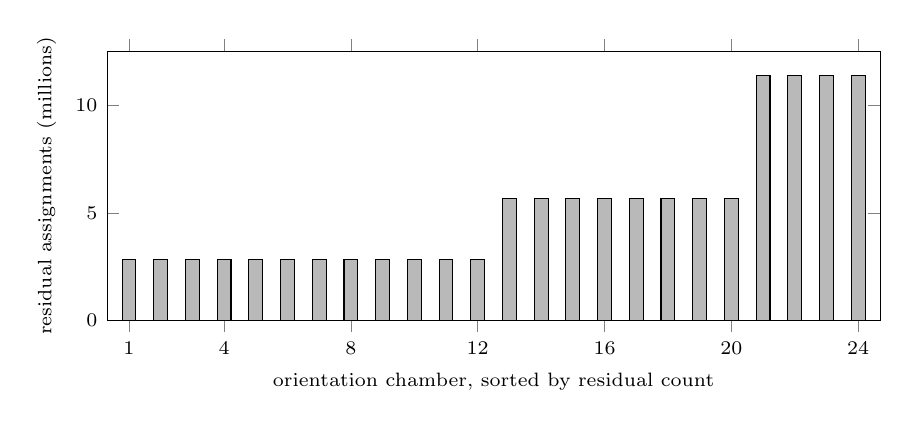
\begin{tikzpicture}
\begin{axis}[ybar, width=0.94\linewidth, height=5cm, ylabel={residual assignments (millions)},
xlabel={orientation chamber, sorted by residual count}, xtick={1,4,8,12,16,20,24}, ymin=0, bar width=5pt,
tick label style={font=\scriptsize}, label style={font=\scriptsize}, enlarge x limits=0.03]
\addplot[fill=gray!55] coordinates {
% BEGIN GENERATED fig-chambers
(1,2.843136) (2,2.843136) (3,2.843136) (4,2.843136) (5,2.843136) (6,2.843136) (7,2.843136) (8,2.843136) (9,2.843136) (10,2.843136) (11,2.843136) (12,2.843136) (13,5.686272) (14,5.686272) (15,5.686272) (16,5.686272) (17,5.686272) (18,5.686272) (19,5.686272) (20,5.686272) (21,11.372544) (22,11.372544) (23,11.372544) (24,11.372544)
% END GENERATED fig-chambers
};
\end{axis}
\end{tikzpicture}
\caption{Residual sign assignments of the free-atom relaxation in each of the 24 feasible orientation chambers,
sorted by count, in millions. The counts take the three values 1, 2 and 4 times 2.843136 million and total 125.097984 million;
no chamber has an empty residual. Data are the stored per-chamber counts of the experiment.}\label{fig:chambers}
\end{figure}

\subsection{The certified interval atlas}

A box of the coordinates $(u,v,p,q)$ is discharged by one of three certificates, all in exact rational interval
arithmetic with outward rounding: (a) \emph{rank}~$\ge3$, some $3\times3$ minor of $J$ excludes zero over the box;
(b) \emph{trap}, a $2\times2$ minor excludes zero over the box (so $R_1$ misses it) and two $3\times3$ minors have a
$2\times2$ gradient subdeterminant excluding zero (so $R_2$ meets it inside a smooth codimension-2 manifold, dimension
2); (c) bisection to a declared depth cap, with residual failures investigated rather than assumed away. Where a limit
is singular (collisions, pair collapses, infinity) the matrix is first put in an analytic chart, with every
singular factor cancelled algebraically, and each chart is gated by a five-point crosscheck against the original matrix.
Symmetry gives a Klein four-group of exact matrix identities (the swap $(u,v,p,q)\mapsto(p,q,u,v)$ and the mirror
$(v,q)\mapsto(-v,-q)$) under which every certificate is invariant\MV.
The statement certified differs from the one that certified numerical methods address. Smale's $\alpha$-theory in exact
rational arithmetic certifies an approximate solution of a polynomial system (Hauenstein and Sottile
\cite{HS12}\Um), and interval certification does the same with interval arithmetic (Breiding, Rose and Timme
\cite{BRT23}\Um); the atlas certifies a rank condition on every box of a region, which is a statement about a
family of matrices and not about a zero, with the same ingredient of rigorous enclosures.

Residual failures of the charts have three origins. A box that contains an excluded face (a collision locus or a
blow-up face) cannot be certified, because the matrix genuinely drops rank there. The face principle resolves it
in two halves: every dyadic shell at positive distance from the face certifies (measured over six halvings), and closed
forms make the rank floor uniform over the shells. Piece 10 treats the corner face (a pair on an axis body), piece 11 the
pair-collapse face and piece 12 the two merge faces\MV. At the pair-collapse face both pairs approach the axis,
$u=\varepsilon a$ and $p=\varepsilon b$ with $a,b>0$ fixed and $\varepsilon\to0$, at fixed heights $v\ne q$. After the
mass columns $m_1$ and $m_2$ are divided by $\varepsilon$ (a positive factor, which does not change the rank) the
$4\times4$ minor on the rows $\{L_{13},L_{15},L_{23},L_{25}\}$ has the closed form
\begin{equation}\label{eq:collapse}
C_2=4ab\,\bigl[\varphi(1-v)\,\varphi(-1-q)-\varphi(-1-v)\,\varphi(1-q)\bigr],\qquad
\varphi(x)=x\Bigl(\frac18-\frac1{|x|^3}\Bigr),
\end{equation}
verified to eight significant digits at $\varepsilon=10^{-7}$ on three rational geometries\MV\
(\path{CC/context/2026-08-02-rank-floor-lemma-dossier.md}, piece~11, lines 782--830). % voice-ok
It vanishes only on a curve of the height plane that does not depend on $a$ and $b$, and on six points of that curve a
$3\times3$ minor with a nonzero limit carries the rank floor\MV. Limited resolution is the second origin: for every chart with failures, the failures share exactly one box
width, the width reached at the shared depth cap, and a deeper cap discharges them\MV. The third origin is mathematics,
once: the cross point below. The face table of the atlas is complete: every chart's matrix evaluated on its own face is
either full rank or closed by pieces 10 to 12\MV.
Table~\ref{tab:atlas} gives the residue accounting.

Figure~\ref{fig:atlas} shows which certificate closes the boxes in the \numAtlasRuns\ covering runs whose stored summary
ends with zero failed boxes and that the accounting lists as certified: the core covering of the shape variety, the four collision-tube
charts, the low-$u$ chart, the far chart, the opposite bi-corner chart and the depth-76 re-run of the fa2b residue. A run is a
binary bisection forest, and a box is counted once, as a leaf, by the certificate that closed it. Pooled over the
runs, \numAtlasLeaves\ leaf boxes are closed, \numAtlasCertShare\ percent of them by a plain rank certificate; the plain share
runs from \numAtlasCertMin\ percent (\numAtlasCertMinRun) to \numAtlasCertMax\ percent (\numAtlasCertMaxRun). The trap
carries up to \numAtlasTrapMax\ percent of the leaves (\numAtlasTrapRun), which is where $R_2$ is only confined and not excluded. Discarded boxes are those a chart sets aside by a declared region test, as the deep chart leaves the quadruple corner to another chart. In the core run,
\numAtlasBall\ boxes are closed by the ball certificate around the exact rank-2 points and are not drawn. The figure does not
show the failed boxes of the runs that did not close, and it does not test the charts themselves, which rest on the
five-point crosscheck against the original matrix.

\begin{figure}[t]\centering
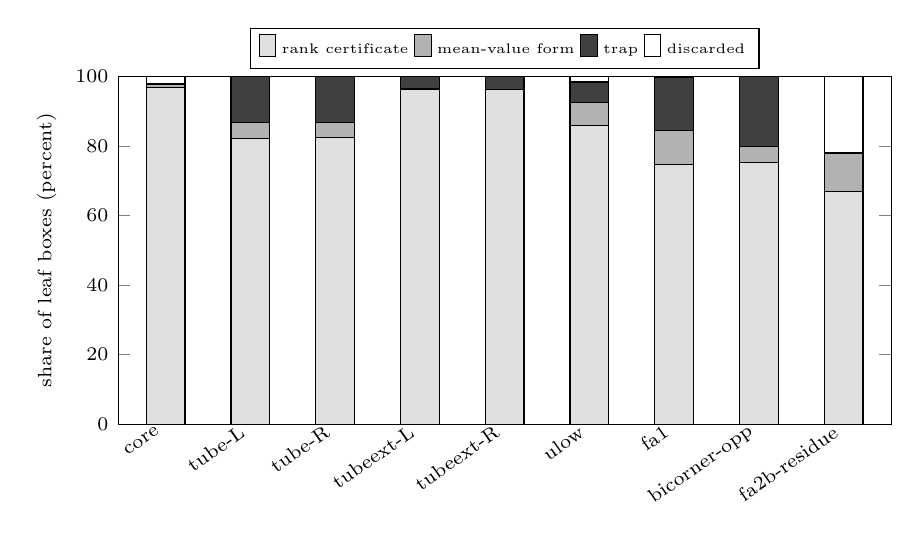
\begin{tikzpicture}
\begin{axis}[ybar stacked, width=0.94\linewidth, height=6cm, ylabel={share of leaf boxes (percent)},
symbolic x coords={%
% BEGIN GENERATED fig-atlas-names
core,tube-L,tube-R,tubeext-L,tubeext-R,ulow,fa1,bicorner-opp,fa2b-residue
% END GENERATED fig-atlas-names
}, xtick=data, x tick label style={rotate=35, anchor=east, font=\scriptsize},
tick label style={font=\scriptsize}, label style={font=\scriptsize}, bar width=14pt, ymin=0, ymax=100,
enlarge x limits=0.07, legend style={font=\tiny, at={(0.5,1.02)}, anchor=south, legend columns=4}]
\addplot[fill=gray!25] coordinates {
% BEGIN GENERATED fig-atlas-cert
(core,96.679) (tube-L,82.194) (tube-R,82.557) (tubeext-L,96.363) (tubeext-R,96.351) (ulow,85.771) (fa1,74.783) (bicorner-opp,75.330) (fa2b-residue,66.972)
% END GENERATED fig-atlas-cert
};
\addplot[fill=gray!60] coordinates {
% BEGIN GENERATED fig-atlas-mv
(core,1.137) (tube-L,4.494) (tube-R,4.189) (tubeext-L,0.000) (tubeext-R,0.000) (ulow,6.693) (fa1,9.684) (bicorner-opp,4.524) (fa2b-residue,11.009)
% END GENERATED fig-atlas-mv
};
\addplot[fill=black!75] coordinates {
% BEGIN GENERATED fig-atlas-trap
(core,0.000) (tube-L,13.312) (tube-R,13.254) (tubeext-L,3.637) (tubeext-R,3.649) (ulow,5.923) (fa1,15.189) (bicorner-opp,20.146) (fa2b-residue,0.000)
% END GENERATED fig-atlas-trap
};
\addplot[fill=white, draw=black] coordinates {
% BEGIN GENERATED fig-atlas-disc
(core,2.181) (tube-L,0.000) (tube-R,0.000) (tubeext-L,0.000) (tubeext-R,0.000) (ulow,1.613) (fa1,0.345) (bicorner-opp,0.000) (fa2b-residue,22.018)
% END GENERATED fig-atlas-disc
};
\legend{rank certificate, mean-value form, trap, discarded}
\end{axis}
\end{tikzpicture}
\caption{Share of the leaf boxes closed by each certificate in the nine covering runs that end with zero failed
boxes: plain rank certificate, mean-value form, trap, and discarded boxes (set aside by the declared region test of the chart). Shares are
read from the stored run summaries; the ball-certified boxes of the core run are too few to show.}\label{fig:atlas}
\end{figure}

\begin{table}[t]\centering\footnotesize
\begin{tabular}{@{}L{3.4cm}L{2.2cm}L{6.9cm}@{}}
\toprule
Residue & Boxes & Disposition \\
\midrule
15 charts & 0 failures & complete \\
fa2b & 200 & discharged at depth 76: 1544 boxes processed, zero failures \\
cb1, cb1f & 5 and 2 & all touch a collision face, closed by piece 10 \\
band & 44 (and 48) & the cross point: a rank-2 degenerate configuration; all 92 boxes are trapped, so $\dim R_2\le2$ holds there \\
m2-L, m2-R & 5824 and 5683 & the quadruple corner: a chart region still open; 6208 boxes of each chart are covered by the collapse chart, the rest by no chart \\
fa2, m1vert-N & retired & replaced by fa2b and by per-entry guards \\
\bottomrule
\end{tabular}
\caption[Residue accounting of the atlas.]{Residue accounting of the atlas of the stratum \path{CC/context/2026-08-20-stratum-theorem-assembly.md}, sections 6b, 6c, 8 and 9.}\label{tab:atlas}
\end{table}

The atlas therefore leaves one mathematical residue, the cross point (next subsection), and one open chart region, the
quadruple corner of the charts m2-L and m2-R. The corner is a defect of the chart and not of the mathematics: the matrix
has rank 3 throughout the open stratum there, the $m_1$ and $m_2$ columns are $O(s)$ while the $m_A$ and $m_B$ columns are
$O(s^{-2})$ (a ratio of exactly $s^3$), and about half of the residual boxes straddle the physical boundary $u_h,p_h\ge0$,
which is not axis aligned. The repair is specified (reparametrize the corner by $(u_h,p_h)$ and divide the two axis-mass
columns by their common factor), and the records do not show it carried out. A first check of the corner compared the
box coordinates of two charts that do not share a parametrization and reported a hole that was not there; the corrected
comparison, through the exact map $c_s=R_c\,s_t$, covers 6208 of the boxes of each chart and leaves the remainder to a
delegation loop between the charts\MV. So the quadruple corner remains open and the covering is complete except for it.

\subsection{The cross point and the finiteness of its family}

The residue of the band chart sits at $v=q=0$, with both mirror pairs at height zero (the doubly symmetric cross).
On that face $\sigma_4$ vanishes identically, so the rank is 3 and each point has a unique mass ray; the cross face carries a
two-parameter family of central configurations. At
$u^{*}=0.6309181371\ldots$, $p^{*}=1.4509074659\ldots$ the rank is exactly 2: $\sigma_3/\sigma_1$ falls in proportion to the
search bracket over thirteen orders of magnitude, and a $3\times4$ system in $(m_1,m_A,m_B,\lambda)$ built from scratch, sharing
no code, confirms $\sigma_3/\sigma_1=8.6\times10^{-34}$ against controls at $8.6\times10^{-3}$, $6.6\times10^{-3}$ and
$5.8\times10^{-2}$\MV. The two-dimensional kernel meets the positive orthant in an arc of width $1.2$ rad, so one
configuration is central for a one-parameter family of positive masses: a degenerate central configuration, with smallest
mutual distance $0.82$. A census over the face (5607 grid points, seven basins) finds exactly one such point\MV.

Symmetry reduces the equations to three scalar conditions, each linear in $(m_1,m_A,m_B,\lambda)$. Eliminating the algebraic
half-powers $C=(u^2+1)^{-3/2}$ and $D=(p^2+1)^{-3/2}$ by resultants leaves two integer polynomials $g_1,g_2$ in $(u,p)$ of 2027 and
936 terms, both vanishing at the point to relative $3.6\times10^{-60}$ and $2.6\times10^{-65}$\MV. The polynomial $g_1$ is the
square of an irreducible polynomial of total degree 40, $g_2$ is irreducible of total degree 56, and $\gcd(g_1,g_2)$ has total
degree 0\MV. The common zero set is therefore zero-dimensional: the degenerate configurations of the doubly symmetric cross family
are finite. With $g_1=h^2$, $h$ irreducible,
\begin{equation}\label{eq:bezout}
\deg h=40,\quad\deg g_2=56,\quad\gcd(h,g_2)=1\ \Longrightarrow\ \#\{h=g_2=0\}\le40\cdot56=2240,
\end{equation}
counted over $\mathbb{C}$ with multiplicity (the resultants may carry extraneous factors, which
places the true set inside their common zero set, the direction finiteness needs)\MV\Dm. The written argument is in
\path{CC/context/2026-08-02-rank-floor-lemma-dossier.md}, lines 1227--1272, % voice-ok
and \path{CC/history/log.md}, lines 822--880 (Round 54), with
the factorizations and the greatest common divisor computed exactly; the statement is not given a theorem environment here because the
irreducibility and coprimality computations are not reproduced in the text.
A numerical identification by integer
relation search found nothing real and was rejected. The scope is the doubly symmetric sub-family (line masses $m_B,m_A,m_A,m_B$,
off-line masses equal), and the statement concerns the \emph{degenerate} configurations, a different question from the one
Dias and Pan answer. The family is not new: it lies in their cross class\Vm, but their theorem excludes a non-generic mass set,
and the configuration is an explicit witness in it (their Proposition~5.2 example is a different configuration).
Whether this specific configuration appears in the wider literature on symmetric central configurations is not checked\Um.

The centred regular pentagon (bodies $1,3,4,5,6$ on a regular pentagon of circumradius 2 centred at body 2) is an exact
rank-2 point with kernel spanned by the free central mass and the equal ring masses, found from interval failures whose
count stayed constant under bisection; with exact gradients of two $3\times3$ minors of rank 2 at that point (piece 8, by the
implicit function theorem) $R_2$ is locally a codimension-2 submanifold near it\MV.

\subsection{The dropped statement and the open questions}

A draft statement for the stratum named the centred pentagon as the sharp degenerate point of the open stratum, and asserted
finiteness of the configurations for all masses outside a proper closed set. It was dropped on 23 August 2026 because it is false
as written: the cross point is a second exact rank-2 point with an admissible mass ray, found on the face $v=q=0$, which the
declaration of the open stratum excludes, so the uniqueness wording fails. The statement is not repeated here.
Three questions have to be settled before any statement is rebuilt:
(1) whether the cross point is the only degenerate point on the closure of the stratum, or only on the cross face (the census
covered the cross face alone, in a bounded window);
(2) whether the open stratum, with pairs at strictly distinct heights, contains a degenerate point besides the centred pentagon;
(3) whether the cross point is known in the literature\Um.
These are open. The atlas, the cases $k=0,1,2,4$ and the reduction of $k=3$ are the established parts; the finiteness statement
for the stratum is not established.

\begin{table}[t]\centering\footnotesize
\begin{tabular}{@{}L{2.0cm}L{4.0cm}L{6.4cm}@{}}
\toprule
Experiment & Instrument & Result \\
\midrule
EXP-015 & Gr\"obner staircase and Singular \texttt{dim()} & shape variety of dimension 5 ungauged, 4 gauged, in one second, two engines agree\MV \\
EXP-016 & exact radical rank at two witnesses & rank 4 at $W_1$ and $W_2$; component decomposition capped\MV \\
EXP-017, 017b, 017c & Gr\"obner bounds for all four loci, $s$-variable model, mod-$p$ triage & every locus bound capped in all three formulations; all ten mod-$p$ cells capped at two primes, so the Gr\"obner route to the loci bounds is closed at the budgets tried\MV \\
EXP-018 & hexagon through the block & hexagon is a stratum configuration with rank exactly 3\MV \\
EXP-019 & Singular $\mathrm{std}$ on the shape ideal plus one minor ($g_4$, $g_3$) & both single-minor cuts capped at 1800 s despite a 32-term increment over a one-second base; all four mod-$p$ cells capped at 300 s, so the Gr\"obner route to the loci bounds is closed at every granularity tried\MV \\
EXP-020 & GF(2) inclusion--exclusion over 24 orientation chambers & 125,097,984 residual sign assignments remain: the free-atom sign relaxation does not close $k=3$, so the geometric couplings are essential\MV \\
EXP-021 & verified covering of the core & 854,317 boxes in 5,096 s, zero residual failures; four pentagon balls (radius $2^{-8}$) carry both certificates; $\dim(R_2\cap\text{core})\le2$, $R_1\cap\text{core}=\emptyset$, $R_0=\emptyset$\MV \\
EXP-022 & collar, tube, collapse, corner and outer coverings; face lemmas 10 to 12 & fifteen charts at zero failures; the residues of Table~\ref{tab:atlas}; the cross point and its exact algebraic system\MV \\
EXP-023 & the stratum with three mirror pairs and no axis body & $6\times3$ matrix of generic rank 3, so central configurations lie on the rank-2 locus; hexagon is rank 2 with the equal-mass kernel; every face is full rank and a compact five-chart atlas passes a seam gate (48,358 samples, zero gaps)\MV; collapse and merge faces still carry face-touching failures, and the blow-up sub-chart is unbuilt \\
\bottomrule
\end{tabular}
\caption{Experiments on the symmetric strata of the six-body problem, from the experiment records.}\label{tab:stratum}
\end{table}

\subsection{The stratum with three mirror pairs (EXP-023)}

The mirror symmetry kills $L_{12},L_{34},L_{56}$ and pairs off the rest, leaving six independent equations over three
masses (a $6\times3$ matrix); its generic rank is 3 (20 of 20 random shapes), so a generic shape admits no masses and the
central configurations of the stratum lie on the rank-at-most-2 locus, a codimension-2 subvariety of the four-dimensional shape space.
The regular hexagon has rank exactly 2 with the equal-mass kernel, which validates the instrument. Unlike the two-pair stratum,
the face matrices are full rank (pair collapse at 27 of 27 sample points, pair merge at 40 of 40, the all-narrow region flat at
$\sigma_3=2.0$), so no face lemma and no chart at infinity is needed. A compact gauge (translation $v_1=0$ and scale
$\max(u_1,u_2,u_3,|v_2|,|v_3|)=1$) replaced two charts that exchanged their residues across arbitrary boundaries. Six collinear
bodies span no triangle, so the Laura--Andoyer matrix is identically zero on the interior collinear locus, which only this stratum
of the family has and which has dimension 2; the equations are vacuous there, and the classical count of Moulton \cite{Moulton10}
settles the collinear shapes, one positive mass ray each\Dm. A lemma piece (piece 13) gives the merge-face rank floor, which
is not bounded below; the merge residue then lies on the surface where one entry vanishes. The stratum still has its collapse and
merge faces open (14,485 collapse failures, all face-touching) and its blow-up sub-chart unbuilt\MV.

\section{The \texorpdfstring{$n=6$}{n=6} attempt (EXP-005)}\label{sec:six}

The screening of Section~\ref{sec:screening} turns the $n=6$ question into a
design problem with two dials. What we have measured is a \emph{tooling}
barrier, characterized on four attempts with \texttt{gfan}~0.7. On the
machine-integer fast path the computation aborts within minutes on a
\emph{detected} overflow (the benign failure mode: \texttt{gfan} raises rather
than returning a wrong answer), and it does so for powers of three and for
powers of two alike, although the latter caps the valuation exponents at 32
instead of 243, so the failure is not a matter of valuation magnitude. On the
arbitrary-precision path, the powers-of-two run died after fifteen wall-hours
(about six cpu-days) on an internal assertion
(\texttt{gfanlib\_hypersurfaceintersection.cpp:505}) in the hypersurface-intersection
code\MV. \texttt{gfan}~0.7 therefore fails at $n=6$ in both arithmetic modes, in two
distinct ways, while the same binary reproduces the published $n=5$ certificates
exactly; \cite{JL25} report their own $n=6$ computation as completing (and
inconclusive on pointedness)\Vm, so their run differed in version, flags, or
valuation. We rebuilt the pipeline on the 0.8beta release, validated it against
our $n=5$ control (exact $f$-vector agreement), and confirmed that it clears
0.7's first failure point\MV.

The 0.8beta runs have not completed. The powers-of-two run on the fast path (\texttt{-{}-bits 64}) has been
paused since 20 August 2026 to free processors for the coverings of Section~\ref{sec:stratum}; it is protected by a
1.2 GB checkpoint written with \texttt{-{}-saveas}, so the pause costs only the work since the last checkpoint. The
powers-of-three run with arbitrary-precision integers (\texttt{-{}-bits 0}) is parked after four launches, none of which
wrote a checkpoint (\path{CC/experiments/EXP-005-n6-prevariety-pow3/PAUSE-NOTE.md})\MV. The measured quantities
(fifteen wall-hours, the assertion location) are kept only in the history log of the problem, as the experiment folder
has no result file. The case $n=6$ therefore remains open here: a completed run would
either extend generic-mass finiteness to $n=6$ or localize the obstruction to
specific comets, data that has not been published for any failed attempt. Resuming it is the only open case of the programme,
and needs a fresh hypothesis and a budget before any run.

\section{The five-body case for all positive masses: claims and a formal audit (EXP-024)}\label{sec:five}

In October 2026 three groups claimed that the planar five-body problem has finitely many central
configurations up to similarity for every positive mass vector: Tomar \cite{Tomar26}, with a Lean~4
formalization and a supplement of certificates; Chen and Tong \cite{ChenTong26}; and Liu and Liu
\cite{LiuLiu26}\Vm. All three complete the Albouy--Kaloshin classification of singular sequences
\cite{AK12} on the exceptional mass set that \cite{AK12} leaves open. The question of the
previous sections for $n=5$ is therefore settled, if these claims hold, and the priority is theirs. None
of the three is refereed. The computer-assisted counts of \cite{MZ26} are an
earlier, separate line: exact class counts for several exceptional mass sets\Vm.

We audited the formalization of \cite{Tomar26} without rebuilding it. Its main theorem,
$\forall m,\ (\forall i,\ 0<m_i)\to\mathrm{FinitelyManyCC}\ m$, is built from a planar configuration
$q:\{1,\dots,5\}\to\mathbb{C}$ with distinct points, the equation
$\lambda m_i(q_i-c)=\sum_{j\ne i}m_im_j(q_i-q_j)/|q_i-q_j|^3$ with $\lambda\in\mathbb{R}$ and
$c\in\mathbb{C}$, and similarity by every map $z\mapsto az+b$ or $z\mapsto a\bar z+b$, $a\ne0$; finitely
many central configurations means finitely many similarity classes. This is the classical statement: the
sign of the force is absorbed by $\lambda$, the value $\lambda=0$ admits no configuration for positive
masses, and counting up to reflections changes counts, not finiteness\Dm. The statement was read in the stored
sources \texttt{System.lean} and \texttt{Basic.lean}\Vm.

A scan of the stored sources and the generated modules (each archive checked against its published SHA-256) searches
for nine textual patterns: \texttt{sorry}, \texttt{admit}, an axiom declaration, \texttt{native\_decide},
\texttt{implemented\_by}, \texttt{extern}, \texttt{ofReduceBool}, \texttt{unsafe} and \texttt{skipKernelTC}. The 2,751 stored
source files were scanned with comments stripped, and the 85,756 generated modules by a raw search including comments. None of the nine
patterns occurs in the formalization; the three hits (all \texttt{unsafe}) are in the exporter used to feed
independent kernels\MV. The scan is a text scan, with a limit: the axiom pattern matches only at the start of a line after
the prefixes \texttt{private}, \texttt{protected} and \texttt{noncomputable}, so an \texttt{axiom} preceded by an
attribute, or a declaration introduced by a metaprogram, would not match; the output of the \texttt{\#print axioms} command
on the main theorem was not obtained. The scan therefore shows that the theorem as formalized is the right statement and that
none of the stored or generated sources contains any of these nine patterns. It does not replace the kernel check, which the
author reports for a full build of about 863 CPU-hours and for two independent kernels, and which we did not reproduce.
The open case for this programme is $n=6$.

\section{Limitations and open items}\label{sec:limits}

\begin{enumerate}
\item The prevariety certificates at $n=4,5$ of Sections~\ref{sec:jl} and \ref{sec:screening} rest on the machine-integer
fast path. The overflow-checked rerun is an open item, not a result; it is not claimed here. Arbitrary precision was used only
in the enrichment grid at $n=4$.
\item The \texttt{gfan} 0.7 tarball and binary hashes are not among the committed artifacts, so that part of the provenance
(Table~\ref{tab:tools}) is unverified; the hashes of every input and output of the screening grid are.
\item Pointedness of every comet is a sufficient condition for dimension zero of the tropical variety; an unpointed comet proves
only that the certificate route does not close. The comet reading depends on \texttt{gfan}'s semantics under
\texttt{-{}-usevaluation}, validated by the count of 257 components.
\item The section probes of Section~\ref{sec:census} are probabilistic and see only the maximum dimension. The completeness of
\texttt{msolve}'s box list is trusted and checked only against the classical counts at $n=3$.
\item The two-pair stratum of the six-body problem has no finiteness statement. The case $k=3$ is not proved, the
quadruple-corner chart region is open, the pair-equality statement is untested by its informative attack, and three
questions on the degenerate points are open.
\item The five-body claims are unrefereed and were not rebuilt; the audit of the Lean statement is a text scan with the limits stated.
\item The enrichment cells at powers of two are read from stored outputs; their wall times were not stored.
\item The stored summary files of several covering runs hold failure counts that differ from the residue accounting of
Table~\ref{tab:atlas} (for example, twenty failed boxes are stored for the collapse chart against zero in the accounting). The
records do not say why, so the accounting follows the assembly record, and Figure~\ref{fig:atlas} uses only the runs whose
stored summary has zero failed boxes and that the accounting lists as certified. Two further runs, of a chart that
reparametrizes the quadruple corner, are stored with zero failed boxes at a depth cap of 48; no record states their coverage of the
corner, so the corner is reported as open and the runs are not used.
\end{enumerate}

\section{Scope and data availability}

The study is replication-first. The finiteness theorems replicated are due
to Hampton--Moeckel, Albouy--Kaloshin, and Jensen--Leykin; the equal-mass
censuses to Moczurad--Zgliczy\'nski. Our measurements (the dimension-blindness
anchors with their exact minimal polynomials and $J$-invariants; the
enrichment law at affine and prevariety level; the screening tables) are
machine facts about known objects, stated with their provenance. The
censuses for two integer-separated mass vectors, which our sympy engine does not
finish, are closed by an independent engine (\texttt{msolve}) with
the sympy layer retained as exact verification, while the $n=4$ torus censuses
and the Dziobek census probes remain capped as reported above. Statements that rest on
a literature source not read in its primary form carry the mark \Um.

The tables, the figure data and the numbers quoted from the records in the figures' discussion are generated from the stored
artifacts by \path{gen_tables.py} next to the source, which
stops when a recomputed cell differs from a stored value or a stored record is missing.

{\raggedright
Code, artifacts and experiment records are available at
\url{https://github.com/fsantibanezleal/CAOS_RESEARCH} under
\path{problems/dynamical-systems/central-configurations/}. The identifiers
EXP-001 to EXP-024 in the section titles and the text denote the experiment
records in its \path{experiments/} folder; each record holds the code, the
artifacts and the result. Tool
versions and binary hashes (\texttt{gfan}, \texttt{msolve}, Singular) are
in Table~\ref{tab:tools} and in the records that use them.\par}

\begin{thebibliography}{99}
\bibitem{Tomar26} T.~S.~Tomar, \emph{Smale's sixth problem for five bodies in the plane, with a proof
formalized in Lean}, arXiv:2610.13100, 2026; supplement doi:10.5281/zenodo.23202861.
\bibitem{ChenTong26} Z.~Chen, Z.~Tong, \emph{Finiteness of planar central configurations of five bodies
for all positive masses: on Smale's sixth problem}, arXiv:2610.16107, 2026.
\bibitem{LiuLiu26} K.~Liu, Y.~Liu, \emph{Finiteness of planar central configurations of five bodies
with positive masses}, arXiv:2610.28168, 2026.
\bibitem{Smale98} S.~Smale, \emph{Mathematical problems for the next century},
Math. Intelligencer \textbf{20} (1998), no.~2, 7--15 (problem text read in the author's second
version dated 7 August 1998).
\bibitem{Chazy18} J.~Chazy, \emph{Sur certaines trajectoires du probl\`eme des
$n$ corps}, Bull. Astron. \textbf{35} (1918), 321--389.
\bibitem{Wintner41} A.~Wintner, \emph{The Analytical Foundations of Celestial
Mechanics}, Princeton University Press, 1941.
\bibitem{HM06} M.~Hampton and R.~Moeckel, \emph{Finiteness of relative
equilibria of the four-body problem}, Invent. Math. \textbf{163} (2006),
289--312.
\bibitem{AK12} A.~Albouy and V.~Kaloshin, \emph{Finiteness of central
configurations of five bodies in the plane}, Ann. of Math. \textbf{176}
(2012), 535--588.
\bibitem{Moeckel01} R.~Moeckel, \emph{Generic finiteness for Dziobek
configurations}, Trans. Amer. Math. Soc. \textbf{353} (2001), 4673--4686.
\bibitem{HJ11} M.~Hampton and A.~N.~Jensen, \emph{Finiteness of spatial
central configurations in the five-body problem}, Celest. Mech. Dyn. Astron.
\textbf{109} (2011), 321--332.
\bibitem{ChangChen23} K.-M.~Chang and K.-C.~Chen, \emph{Toward finiteness of
central configurations for the planar six-body problem by symbolic
computations. (I) Determine diagrams and orders}, J. Symbolic Comput.
\textbf{123} (2024), 102277; preprint of the programme: arXiv:2303.02853. (A
second part, on mass relations, is announced in the same programme; we cite
only the part whose bibliographic data we verified from a primary source.)
\bibitem{JL25} A.~Jensen and A.~Leykin, \emph{Smale's 6th problem for generic
masses}, arXiv:2301.02305v2 (2025).
\bibitem{MZ19} M.~Moczurad and P.~Zgliczy\'nski, \emph{Central configurations
in planar $n$-body problem with equal masses for $n=5,6,7$}, Celest. Mech.
Dyn. Astron. \textbf{131} (2019); arXiv:1812.07279.
\bibitem{DP18} T.~Dias and B.-Y.~Pan, \emph{Generic finiteness for a class of
symmetric planar central configurations of the six-body problem and the
six-vortex problem}, arXiv:1811.08681 (2018).
\bibitem{Roberts99} G.~E.~Roberts, \emph{A continuum of relative equilibria in
the five-body problem}, Phys. D \textbf{127} (1999), 141--145 (read in the author
preprint mp\_arc 98-554).
\bibitem{AC98} A.~Albouy and A.~Chenciner, \emph{Le probl\`eme des $n$ corps
et les distances mutuelles}, Invent. Math. \textbf{131} (1998), 151--184.
\bibitem{Moulton10} F.~R.~Moulton, \emph{The straight line solutions of the
problem of $n$ bodies}, Ann. of Math. \textbf{12} (1910), 1--17.
\bibitem{Euler67} L.~Euler, \emph{De motu rectilineo trium corporum se mutuo attrahentium}, 1767; cited
through the secondary literature, the primary printing was not read.
\bibitem{Lagrange72} J.-L.~Lagrange, \emph{Essai sur le probl\`eme des trois corps}, 1772; cited through the
secondary literature, the primary printing was not read.
\bibitem{Dziobek00} O.~Dziobek, \emph{\"Uber einen merkw\"urdigen Fall des Vielk\"orperproblems}, Astron. Nachr.
\textbf{152} (1900), 33--46, doi:10.1002/asna.19001520302 (bibliographic data confirmed on Crossref; the
paper was not read).
\bibitem{Dias17} T.~Dias, \emph{New equations for central configurations and generic finiteness}, Proc. Amer. Math. Soc.
\textbf{145} (2017), 3069--3084, doi:10.1090/proc/13427.
\bibitem{Dias26} T.~Dias, \emph{The Veronese geometry of Dziobek configurations and generic finiteness for homogeneous
potentials}, arXiv:2601.07962, 2026 (abstract read).
\bibitem{MZ20} M.~Moczurad and P.~Zgliczy\'nski, \emph{Central configurations in the spatial $n$-body problem for
$n=5,6$ with equal masses}, Celest. Mech. Dyn. Astron. \textbf{132} (2020), no.~11--12,
doi:10.1007/s10569-020-09993-1; arXiv:2006.06768 (abstract read).
\bibitem{MZ26} M.~Moczurad and P.~Zgliczy\'nski, \emph{Central configurations with unequal masses: finiteness in several
exceptional cases of five bodies}, arXiv:2601.01165, 2026 (abstract read).
\bibitem{Jensen24} A.~N.~Jensen, \emph{Dynamic decomposition of tropical prevarieties for celestial mechanics}, in
Mathematical Software, ICMS 2024, Lecture Notes in Comput. Sci., Springer, 2024, 313--321,
doi:10.1007/978-3-031-64529-7\_34 (cited through \cite{JL25}; not read).
\bibitem{BG84} R.~Bieri and J.~R.~J.~Groves, \emph{The geometry of the set of characters induced by valuations},
J. reine angew. Math. \textbf{347} (1984), 168--195, doi:10.1515/crll.1984.347.168 (cited through \cite{JL25}; not read).
\bibitem{Payne09} S.~Payne, \emph{Fibers of tropicalization}, Math. Z. \textbf{262} (2009), 301--311,
doi:10.1007/s00209-008-0374-x (cited through \cite{JL25}; not read; an erratum, Math. Z. \textbf{272} (2012),
1403--1406, doi:10.1007/s00209-012-1080-2, exists and was not read).
\bibitem{MS15} D.~Maclagan and B.~Sturmfels, \emph{Introduction to Tropical Geometry}, Graduate Studies in
Mathematics \textbf{161}, American Mathematical Society, 2015, doi:10.1090/gsm/161 (cited through \cite{JL25}; not read).
\bibitem{HS12} J.~D.~Hauenstein and F.~Sottile, \emph{Algorithm 921: alphaCertified: certifying solutions to
polynomial systems}, ACM Trans. Math. Software \textbf{38} (2012), no.~4, doi:10.1145/2331130.2331136;
arXiv:1011.1091 (abstract level only).
\bibitem{BRT23} P.~Breiding, K.~Rose and S.~Timme, \emph{Certifying zeros of polynomial systems using interval
arithmetic}, ACM Trans. Math. Software \textbf{49} (2023), no.~1, doi:10.1145/3580277; arXiv:2011.05000
(abstract level only).
\bibitem{Simo78} C.~Sim\'o, \emph{Relative equilibrium solutions in the four body problem}, Celest. Mech.
\textbf{18} (1978), 165--184, doi:10.1007/BF01228714 (cited through \cite{MZ19}; not read).
\bibitem{Albouy96} A.~Albouy, \emph{The symmetric central configurations of four equal masses}, in Hamiltonian
Dynamics and Celestial Mechanics, Contemp. Math. \textbf{198}, Amer. Math. Soc., 1996, 131--135,
doi:10.1090/conm/198/02494 (cited through \cite{MZ19}; not read).
\end{thebibliography}

\end{document}
